\documentclass[aspectratio=169]{beamer}

% Persian support
\usepackage{xepersian}
\settextfont[Path={./font/}, Scale=1.2]{IRLotus}
\setlatintextfont[Scale=1]{Times New Roman}

% Graphics
\usepackage{graphicx}

% Theme
\usetheme{Madrid}
\usecolortheme{default}

% Custom colors for highlighting
\definecolor{important}{RGB}{200,0,0}
\definecolor{highlight}{RGB}{0,100,200}
\definecolor{success}{RGB}{0,150,0}

% Title information
\title{گزارش پروژه نهایی}
\subtitle{درس مبانی هوش مصنوعی - FIS4041}
\author{نیکی مهدیان \and مبینا یوسفی مقدم}
\institute{دانشگاه}
\date{\today}

% Remove navigation symbols
\setbeamertemplate{navigation symbols}{}

\begin{document}

% Title slide
\begin{frame}
\titlepage
\end{frame}

% Outline
\begin{frame}{فهرست مطالب}
\tableofcontents
\end{frame}

% ============================================
% SECTION 1: INTRODUCTION
% ============================================
\section{مقدمه}

\begin{frame}{معرفی پروژه}
\begin{itemize}
\item پروژه شامل چهار بخش اصلی:
\begin{enumerate}
\item انتخاب ویژگی با الگوریتم‌های بهینه‌سازی (PSO و GA)
\item خوشه‌بندی داده‌های مشتریان مرکز خرید
\item بررسی نظری الگوریتم یادگیری Q
\item پیاده‌سازی کامل خط لوله یادگیری ماشین
\end{enumerate}
\item استفاده از داده‌های واقعی
\item پیاده‌سازی جامع از نظریه تا عمل
\end{itemize}
\end{frame}

% ============================================
% SECTION 2: QUESTION 1
% ============================================
\section{سوال ۱: انتخاب ویژگی}

\begin{frame}{انتخاب ویژگی - مسئله}
\begin{block}{هدف}
یافتن زیرمجموعه بهینه از ویژگی‌ها برای پیش‌بینی وضعیت وام
\end{block}
\begin{itemize}
\item مجموعه داده: ۱۱ ویژگی، ۴۹۹ نمونه
\item استفاده از دو الگوریتم بهینه‌سازی:
\begin{itemize}
\item \textbf{PSO} (Particle Swarm Optimization)
\item \textbf{GA} (Genetic Algorithm)
\end{itemize}
\item تابع هدف: تعادل بین دقت و تعداد ویژگی‌ها
\end{itemize}
\end{frame}

\begin{frame}{نتایج PSO}
\begin{columns}
\column{0.5\textwidth}
\begin{block}{پارامترها}
\begin{itemize}
\item تعداد ذرات: ۵۰
\item تعداد تکرار: ۱۰۰
\item وزن اینرسی: ۰.۹
\item پارامتر شناختی: ۰.۵
\item پارامتر اجتماعی: ۰.۳
\end{itemize}
\end{block}

\column{0.5\textwidth}
\begin{block}{نتایج}
\begin{itemize}
\item همگرایی در تکرار ۷
\item ویژگی انتخاب شده: \textcolor{important}{\textbf{Credit\_History}}
\item دقت: \textcolor{highlight}{\textbf{۸۰.۶۷\%}}
\item کاهش ابعاد: \textcolor{success}{\textbf{۹۰.۹\%}}
\end{itemize}
\end{block}
\end{columns}
\end{frame}

\begin{frame}{نتایج GA}
\begin{columns}
\column{0.5\textwidth}
\begin{block}{پارامترها}
\begin{itemize}
\item اندازه جمعیت: ۵۰
\item تعداد نسل: ۵۰
\item احتمال تقاطع: ۰.۹
\item احتمال جهش: ۰.۱
\item انتخاب: Tournament
\end{itemize}
\end{block}

\column{0.5\textwidth}
\begin{block}{نتایج}
\begin{itemize}
\item همگرایی در نسل ۳
\item ویژگی انتخاب شده: \textcolor{important}{\textbf{Credit\_History}}
\item دقت: \textcolor{highlight}{\textbf{۸۰.۶۷\%}}
\item کاهش ابعاد: \textcolor{success}{\textbf{۹۰.۹\%}}
\end{itemize}
\end{block}
\end{columns}
\end{frame}

\begin{frame}{مقایسه PSO و GA}
\begin{table}[h]
\centering
\small
\begin{tabular}{|c|c|c|}
\hline
\textbf{معیار} & \textbf{PSO} & \textbf{GA} \\
\hline
سرعت همگرایی & تکرار ۷ & نسل ۳ \\
\hline
ویژگی انتخاب شده & Credit\_History & Credit\_History \\
\hline
دقت & ۸۰.۶۷\% & ۸۰.۶۷\% \\
\hline
کاهش ابعاد & ۹۰.۹\% & ۹۰.۹\% \\
\hline
\end{tabular}
\end{table}

\begin{alertblock}{نتیجه کلیدی}
هر دو الگوریتم به جواب یکسان رسیدند که نشان‌دهنده پایداری و صحت نتیجه است.
\end{alertblock}
\end{frame}

\begin{frame}{مقایسه همگرایی PSO و GA}
\begin{center}
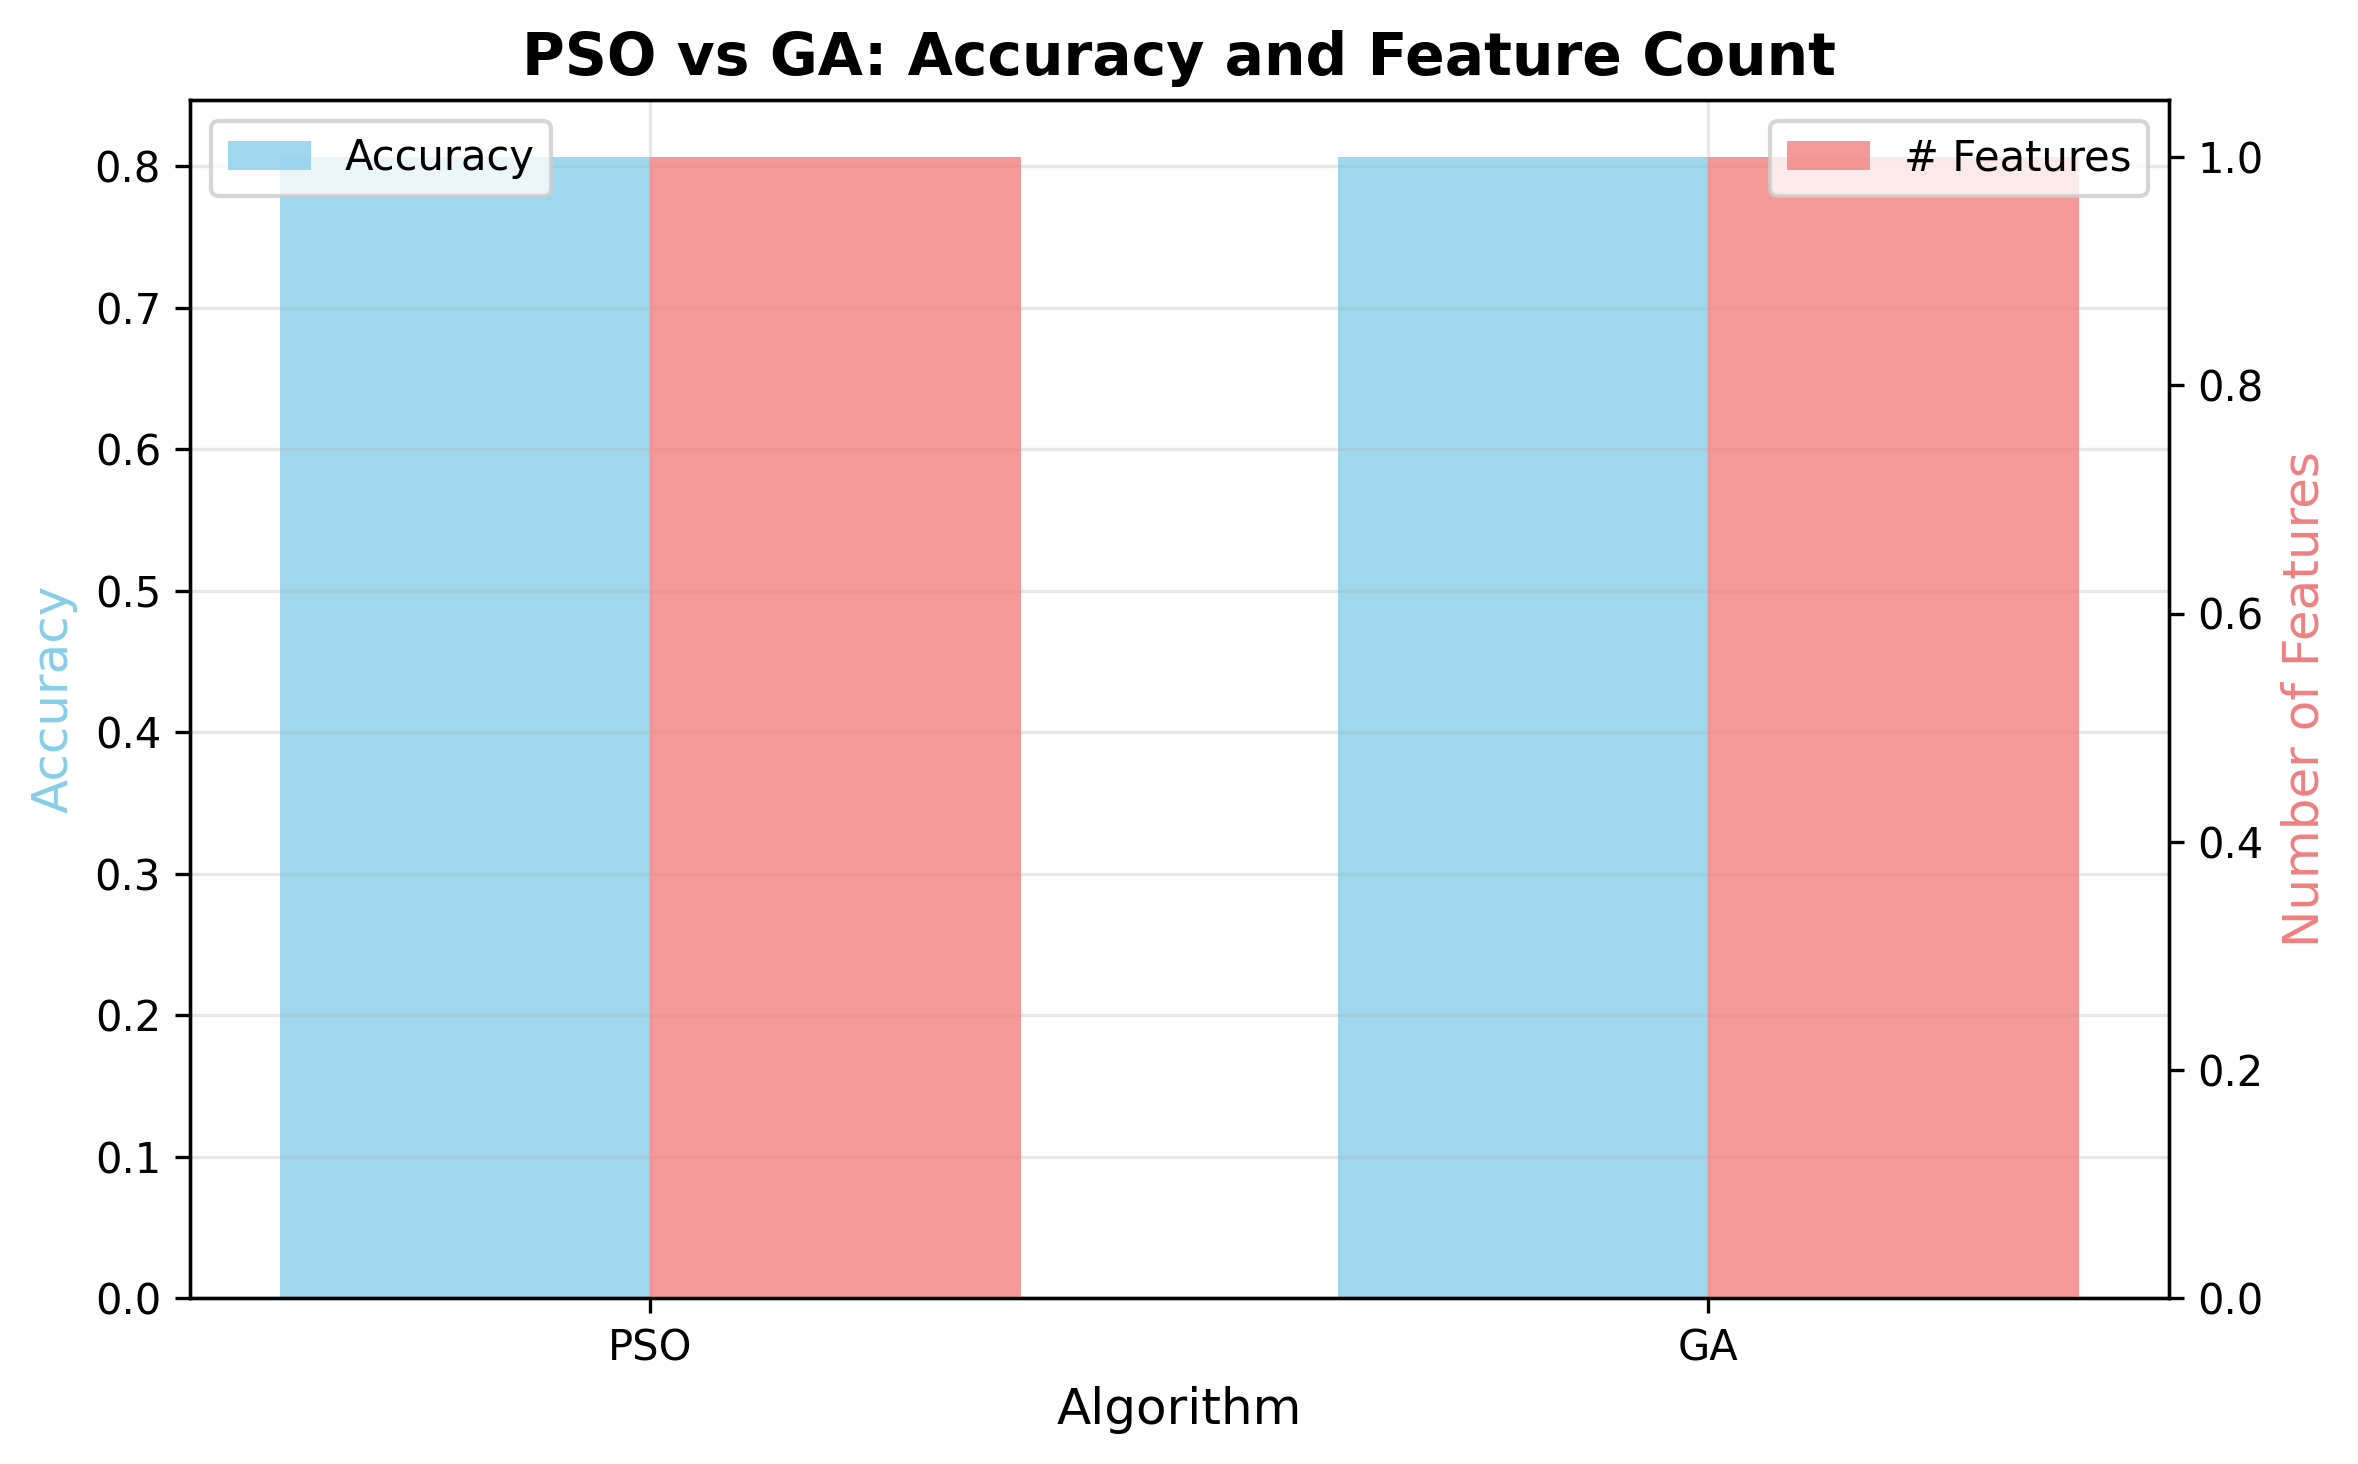
\includegraphics[width=0.8\textwidth]{img/question1_comparison.png}
\end{center}
\begin{block}{تحلیل}
\begin{itemize}
\item هر دو الگوریتم به سرعت همگرا شدند
\item GA سریع‌تر همگرا شد (نسل ۳ در مقابل تکرار ۷)
\item هر دو به جواب بهینه یکسان رسیدند
\end{itemize}
\end{block}
\end{frame}

% ============================================
% SECTION 3: QUESTION 2
% ============================================
\section{سوال ۲: خوشه‌بندی}

\begin{frame}{خوشه‌بندی - مسئله}
\begin{block}{هدف}
تقسیم‌بندی مشتریان مرکز خرید به گروه‌های همگن برای استراتژی بازاریابی
\end{block}
\begin{itemize}
\item مجموعه داده: ۲۰۰ مشتری، ۳ ویژگی
\begin{itemize}
\item سن (Age)
\item درآمد سالانه (Annual Income)
\item امتیاز خرج کردن (Spending Score)
\end{itemize}
\item سه الگوریتم مورد بررسی:
\begin{itemize}
\item K-Means
\item Agglomerative Hierarchical
\item DBSCAN
\end{itemize}
\end{itemize}
\end{frame}

\begin{frame}{نتایج K-Means}
\begin{columns}
\column{0.5\textwidth}
\begin{block}{تحلیل K از ۲ تا ۱۰}
\begin{itemize}
\item K بهینه: \textbf{۶}
\item Inertia: ۱۵۱.۵۷
\item Silhouette Score: \textbf{۰.۴۲۷۴}
\end{itemize}
\end{block}

\begin{block}{توجیه}
\begin{itemize}
\item بالاترین Silhouette Score
\item نقطه آرنج در نمودار Inertia
\item تعادل بین کیفیت و تعداد خوشه‌ها
\end{itemize}
\end{block}

\column{0.5\textwidth}
\begin{block}{مزایا}
\begin{itemize}
\item خوشه‌های کروی و فشرده
\item سریع و کارآمد
\item مناسب برای داده‌های با ساختار کروی
\end{itemize}
\end{block}

\begin{block}{محدودیت‌ها}
\begin{itemize}
\item نیاز به تعیین K از ابتدا
\item فقط خوشه‌های کروی
\end{itemize}
\end{block}
\end{columns}
\end{frame}

\begin{frame}{نتایج Agglomerative Clustering}
\begin{columns}
\column{0.5\textwidth}
\begin{block}{روش‌های پیوند}
\begin{itemize}
\item Single: -۰.۰۴۲۸
\item Complete: ۰.۳۷۴۶
\item Average: ۰.۳۸۹۶
\item \textbf{Ward: ۰.۴۲۰۱} ✓
\end{itemize}
\end{block}

\begin{block}{Ward Linkage}
\begin{itemize}
\item حداقل کردن واریانس درون خوشه‌ای
\item خوشه‌های فشرده و کروی
\item مناسب برای داده‌های کروی
\end{itemize}
\end{block}

\column{0.5\textwidth}
\begin{block}{مزایا}
\begin{itemize}
\item ساختار سلسله‌مراتبی
\item نیازی به تعیین K از ابتدا نیست
\item مناسب برای داده‌های کوچک تا متوسط
\end{itemize}
\end{block}

\begin{block}{محدودیت‌ها}
\begin{itemize}
\item پیچیدگی محاسباتی بالا
\item مناسب برای داده‌های بزرگ نیست
\end{itemize}
\end{block}
\end{columns}
\end{frame}

\begin{frame}{نتایج DBSCAN}
\begin{columns}
\column{0.5\textwidth}
\begin{block}{جستجوی شبکه}
\begin{itemize}
\item eps: [0.2, 0.4, 0.6, 0.8, 1.0]
\item min\_samples: [3, 5, 10]
\item تعداد پیکربندی: ۱۵
\end{itemize}
\end{block}

\begin{block}{بهترین پیکربندی}
\begin{itemize}
\item eps: \textbf{۰.۶}
\item min\_samples: \textbf{۱۰}
\item تعداد خوشه‌ها: ۴
\item نقاط نویز: ۶۶ (۳۳\%)
\end{itemize}
\end{block}

\column{0.5\textwidth}
\begin{block}{نتایج}
\begin{itemize}
\item Silhouette Score: \textcolor{important}{\textbf{۰.۵۲۹۶}}
\item \textcolor{success}{\textbf{بهترین عملکرد}} در بین همه الگوریتم‌ها
\item شناسایی خوشه‌های غیرکروی
\item تشخیص طبیعی نقاط نویز
\end{itemize}
\end{block}

\begin{block}{مزایا}
\begin{itemize}
\item نیازی به تعیین K نیست
\item خوشه‌های با شکل دلخواه
\item مقاوم به داده‌های پرت
\end{itemize}
\end{block}
\end{columns}
\end{frame}

\begin{frame}{مقایسه الگوریتم‌های خوشه‌بندی}
\begin{table}[h]
\centering
\small
\begin{tabular}{|c|c|c|}
\hline
\textbf{الگوریتم} & \textbf{Silhouette Score} & \textbf{تعداد خوشه‌ها} \\
\hline
K-Means (K=6) & ۰.۴۲۷۴ & ۶ \\
\hline
Agglomerative (Ward) & ۰.۴۲۰۱ & ۶ \\
\hline
\textbf{DBSCAN} & \textbf{۰.۵۲۹۶} & \textbf{۴} \\
\hline
\end{tabular}
\end{table}

\begin{alertblock}{نتیجه کلیدی}
DBSCAN با امتیاز Silhouette برابر \textcolor{important}{\textbf{۰.۵۲۹۶}} بهترین عملکرد را داشت و توانست خوشه‌های غیرکروی را شناسایی کند و نقاط نویز را به طور طبیعی تشخیص دهد.
\end{alertblock}
\end{frame}

\begin{frame}{تجسم خوشه‌بندی‌ها}
\begin{center}
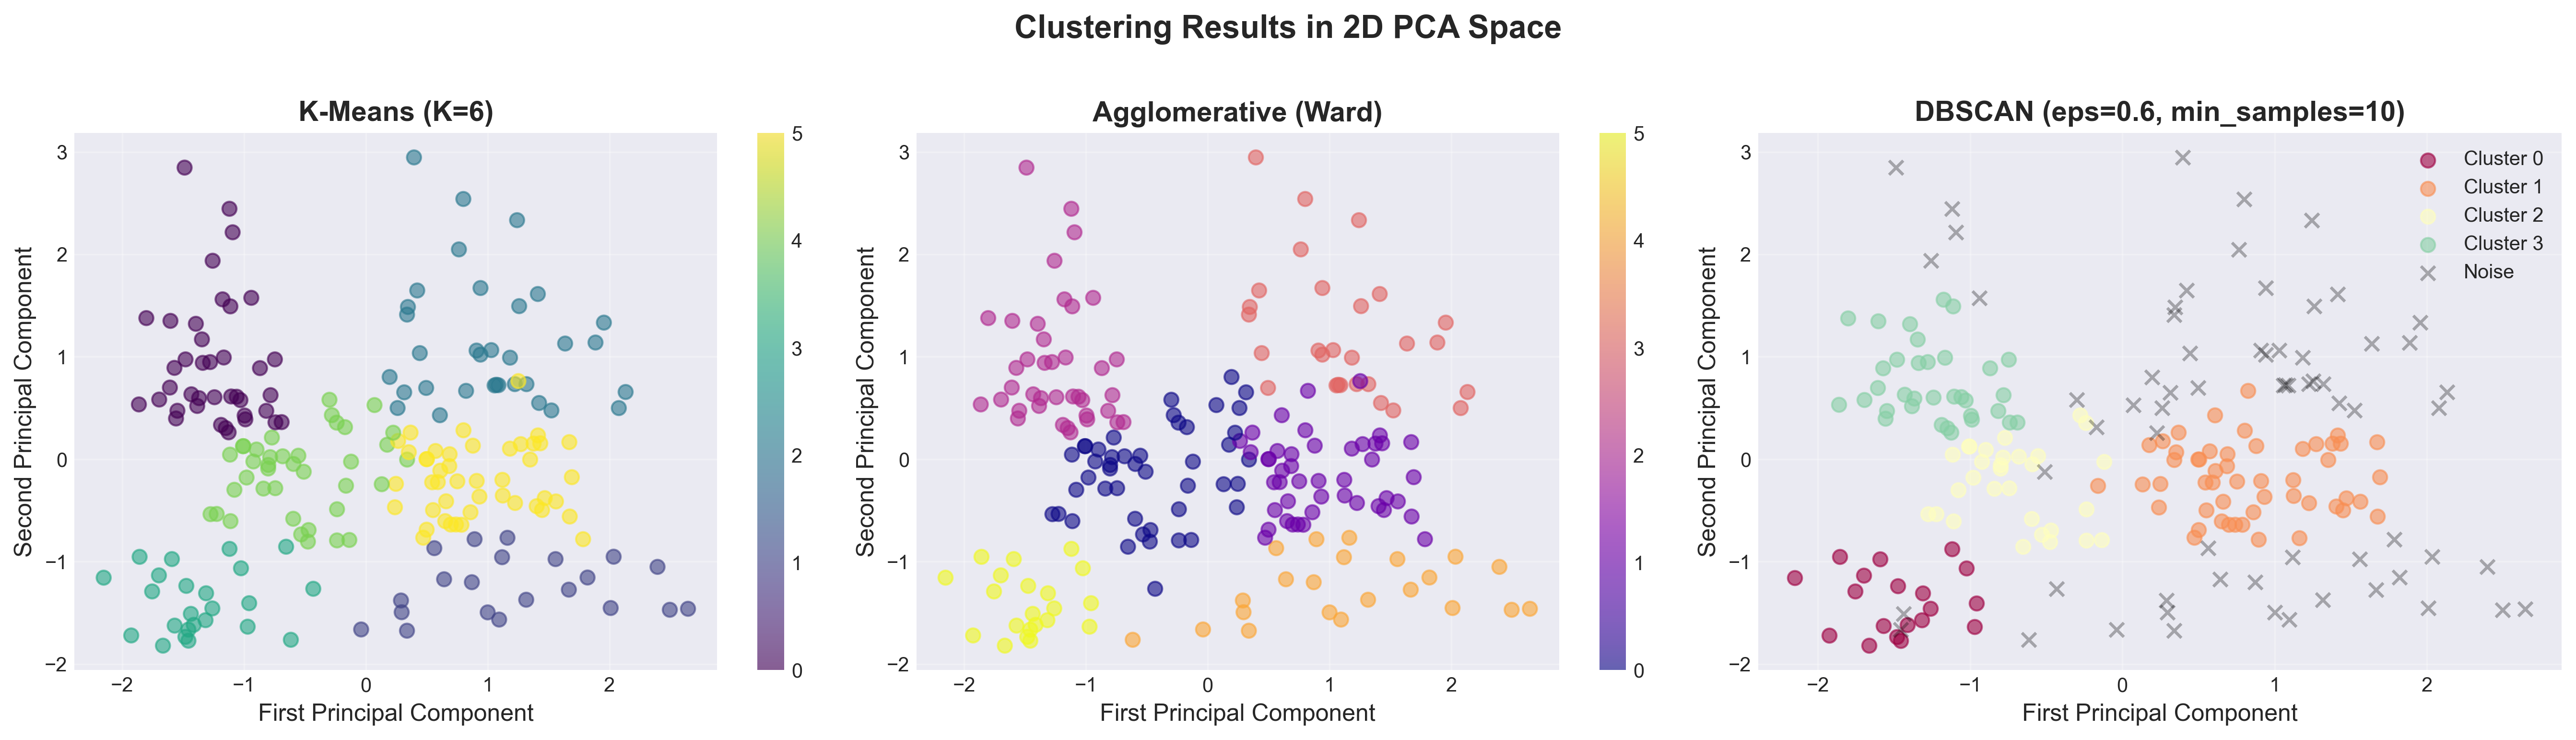
\includegraphics[width=0.9\textwidth]{img/question2_clustering_visualization.png}
\end{center}
\begin{block}{مشاهده}
\begin{itemize}
\item K-Means: خوشه‌های کروی و فشرده
\item Agglomerative: ساختار سلسله‌مراتبی
\item DBSCAN: خوشه‌های غیرکروی و نقاط نویز (سیاه)
\end{itemize}
\end{block}
\end{frame}

% ============================================
% SECTION 4: QUESTION 3
% ============================================
\section{سوال ۳: یادگیری Q}

\begin{frame}{یادگیری Q - معادله}
\begin{block}{معادله به‌روزرسانی Q}
\begin{equation*}
Q_{t+1}(s_t, a_t) = (1 - \alpha) Q_t(s_t, a_t) + \alpha(r_t + \gamma \max_{a'} Q_t(s_{t+1}, a'))
\end{equation*}
\end{block}

\begin{columns}
\column{0.5\textwidth}
\begin{block}{اجزای معادله}
\begin{itemize}
\item $(1-\alpha)Q_t$: حفظ اطلاعات قدیمی
\item $\alpha r_t$: پاداش فوری
\item $\alpha\gamma\max Q_{t+1}$: ارزش آینده تنزیل شده
\end{itemize}
\end{block}

\column{0.5\textwidth}
\begin{block}{پارامترها}
\begin{itemize}
\item $\alpha$: نرخ یادگیری (۰.۱ تا ۰.۵)
\item $\gamma$: عامل تنزیل (۰.۹ تا ۰.۹۹)
\item $\epsilon$: احتمال اکتشاف (۰.۹ تا ۰.۰۱)
\end{itemize}
\end{block}
\end{columns}
\end{frame}

\begin{frame}{یادگیری Off-Policy}
\begin{block}{تعریف}
یادگیری Q یک الگوریتم \textbf{off-policy} است.
\end{block}

\begin{columns}
\column{0.5\textwidth}
\begin{block}{سیاست رفتار}
\begin{itemize}
\item سیاستی که برای انتخاب عمل استفاده می‌شود
\item مثال: $\epsilon$-greedy
\item اجازه اکتشاف می‌دهد
\end{itemize}
\end{block}

\column{0.5\textwidth}
\begin{block}{سیاست هدف}
\begin{itemize}
\item سیاست بهینه که یاد گرفته می‌شود
\item همیشه عمل حریصانه را انتخاب می‌کند
\item از $\max Q$ استفاده می‌کند
\end{itemize}
\end{block}
\end{columns}

\begin{block}{نکته کلیدی}
الگوریتم می‌تواند سیاست بهینه را یاد بگیرد در حالی که از سیاست دیگری برای اکتشاف استفاده می‌کند.
\end{block}
\end{frame}

\begin{frame}{مثال محاسبه Q}
\begin{block}{مقدارهای داده شده}
\begin{itemize}
\item $Q(s_0, a_1) = 0.0$ (مقدار اولیه)
\item انتقال: $(s_0, a_1, r=+2.0, s_1)$
\item $\max_{a'} Q(s_1, a') = 1.5$
\item $\alpha = 0.2$، $\gamma = 0.9$
\end{itemize}
\end{block}

\begin{block}{مراحل محاسبه}
\begin{enumerate}
\item پاداش فوری: $r_t = 2.0$
\item ارزش آینده: $\gamma \times \max Q = 0.9 \times 1.5 = 1.35$
\item هدف TD: $2.0 + 1.35 = 3.35$
\item Q جدید: $(1-0.2) \times 0.0 + 0.2 \times 3.35 = 0.67$
\end{enumerate}
\end{block}

\begin{block}{پاسخ نهایی}
$Q_{t+1}(s_0, a_1) = 0.6700$
\end{block}
\end{frame}

\begin{frame}{مسائل همگرایی}
\begin{columns}
\column{0.5\textwidth}
\begin{block}{مشکل ۱: نرخ یادگیری نامناسب}
\begin{itemize}
\item \textbf{خیلی بالا}: نوسان و واگرایی
\item \textbf{خیلی پایین}: همگرایی کند
\end{itemize}
\end{block}

\begin{block}{راه‌حل‌ها}
\begin{itemize}
\item برنامه زمان‌بندی تطبیقی
\item $\alpha(s,a) = 1/(1+N(s,a))$
\item کاهش تدریجی نرخ یادگیری
\end{itemize}
\end{block}

\column{0.5\textwidth}
\begin{block}{مشکل ۲: اکتشاف ناکافی}
\begin{itemize}
\item گیر کردن در بهینه‌های محلی
\item همگرایی به سیاست زیربهینه
\end{itemize}
\end{block}

\begin{block}{راه‌حل‌ها}
\begin{itemize}
\item برنامه زمان‌بندی کاهش $\epsilon$
\item مقداردهی اولیه خوش‌بینانه
\item اکتشاف Boltzmann (Softmax)
\end{itemize}
\end{block}
\end{columns}
\end{frame}

% ============================================
% SECTION 5: FINAL PROJECT
% ============================================
\section{پروژه نهایی: خط لوله ML}

\begin{frame}{پروژه نهایی - معرفی}
\begin{block}{هدف}
پیاده‌سازی کامل خط لوله یادگیری ماشین برای پیش‌بینی وضعیت وام
\end{block}

\begin{itemize}
\item مجموعه داده: ۶۱۴ نمونه، ۱۱ ویژگی
\item توزیع کلاس: ۶۸.۷\% تأیید شده، ۳۱.۳\% رد شده
\item هفت بخش اصلی:
\begin{enumerate}
\item معرفی مسئله و داده
\item پیش‌پردازش داده
\item کاهش ابعاد
\item انتخاب و آموزش مدل
\item تنظیم ابرپارامترها
\item ارزیابی و قابلیت تکرار
\item تجسم و تحلیل
\end{enumerate}
\end{itemize}
\end{frame}

\begin{frame}{بخش ۱: پیش‌پردازش داده}
\begin{columns}
\column{0.5\textwidth}
\begin{block}{مدیریت مقادیر گم‌شده}
\begin{itemize}
\item مجموعاً ۱۲۷ مقدار گم‌شده
\item متغیرهای دسته‌ای: کدگذاری با مد
\item متغیرهای عددی: کدگذاری با میانه
\end{itemize}
\end{block}

\begin{block}{کدگذاری متغیرهای دسته‌ای}
\begin{itemize}
\item استفاده از LabelEncoder
\item تبدیل به فرمت عددی
\item ۶ ویژگی دسته‌ای کدگذاری شد
\end{itemize}
\end{block}

\column{0.5\textwidth}
\begin{block}{درمان داده‌های پرت}
\begin{itemize}
\item روش: IQR (Interquartile Range)
\item درمان: Capping (Winsorization)
\item حفظ داده‌ها به جای حذف
\end{itemize}
\end{block}

\begin{block}{مقیاس‌گذاری}
\begin{itemize}
\item استفاده از StandardScaler
\item فرمول: $z = (x - \mu) / \sigma$
\item همه ویژگی‌ها: میانگین ۰، انحراف معیار ۱
\end{itemize}
\end{block}
\end{columns}
\end{frame}

\begin{frame}{بخش ۲: کاهش ابعاد}
\begin{table}[h]
\centering
\small
\begin{tabular}{|c|c|c|}
\hline
\textbf{روش} & \textbf{مؤلفه‌ها} & \textbf{دقت} \\
\hline
PCA & ۵ & ۶۹.۷۳\% \\
\hline
LDA & ۱ & ۵۶.۷۶\% \\
\hline
t-SNE & ۲ & فقط تجسم \\
\hline
\end{tabular}
\end{table}

\begin{block}{نتیجه}
\begin{itemize}
\item PCA با ۵ مؤلفه: ۸۸.۹۲\% واریانس توضیح داده شده
\item استفاده از PCA برای تجسم
\item مدل‌ها روی فضای اصلی آموزش داده شدند
\end{itemize}
\end{block}
\end{frame}

\begin{frame}{بخش ۳: انتخاب مدل}
\begin{columns}
\column{0.5\textwidth}
\begin{block}{Random Forest}
\begin{itemize}
\item روش مجموعه‌ای مبتنی بر درخت
\item مقاوم به داده‌های پرت
\item اهمیت ویژگی‌ها
\item استفاده از class\_weight='balanced'
\end{itemize}
\end{block}

\begin{block}{Gradient Boosting}
\begin{itemize}
\item یادگیری ترتیبی
\item عملکرد بالاتر
\item یادگیری الگوهای پیچیده
\end{itemize}
\end{block}

\column{0.5\textwidth}
\begin{block}{SVM}
\begin{itemize}
\item برای مقایسه
\item نیاز به مقیاس‌گذاری
\item عملکرد متوسط
\end{itemize}
\end{block}

\begin{block}{انتخاب نهایی}
\begin{itemize}
\item Random Forest و Gradient Boosting
\item به عنوان مدل‌های اصلی انتخاب شدند
\end{itemize}
\end{block}
\end{columns}
\end{frame}

\begin{frame}{بخش ۴: تنظیم ابرپارامترها}
\begin{columns}
\column{0.5\textwidth}
\begin{block}{Random Forest}
\begin{itemize}
\item روش: Grid Search
\item CV: ۵-fold
\item بهترین پارامترها:
\begin{itemize}
\item max\_depth: ۱۰
\item n\_estimators: ۲۰۰
\item min\_samples\_split: ۱۰
\item min\_samples\_leaf: ۴
\end{itemize}
\end{itemize}
\end{block}

\column{0.5\textwidth}
\begin{block}{Gradient Boosting}
\begin{itemize}
\item روش: Random Search
\item CV: ۵-fold
\item بهترین پارامترها:
\begin{itemize}
\item n\_estimators: ۵۰
\item learning\_rate: ۰.۰۱
\item max\_depth: ۷
\item min\_samples\_split: ۱۰
\end{itemize}
\end{itemize}
\end{block}
\end{columns}
\end{frame}

\begin{frame}{بخش ۵: نتایج ارزیابی}
\begin{table}[h]
\centering
\small
\begin{tabular}{|c|c|c|}
\hline
\textbf{معیار} & \textbf{Random Forest} & \textbf{Gradient Boosting} \\
\hline
Accuracy & ۶۷.۴۸\% & ۶۷.۴۸\% \\
\hline
Precision & \textbf{۷۱.۸۴\%} & ۶۸.۹۱\% \\
\hline
Recall & ۸۷.۰۶\% & \textbf{۹۶.۴۷\%} \\
\hline
F1-Score & ۷۸.۷۲\% & \textbf{۸۰.۳۹\%} \\
\hline
ROC-AUC & ۰.۵۱۳۸ & ۰.۵۴۵۵ \\
\hline
\end{tabular}
\end{table}

\begin{block}{تحلیل نتایج}
\begin{itemize}
\item Gradient Boosting: بهترین F1-Score (\textcolor{highlight}{\textbf{۸۰.۳۹\%}}) و Recall (\textcolor{success}{\textbf{۹۶.۴۷\%}})
\item Random Forest: بهترین Precision (\textcolor{important}{\textbf{۷۱.۸۴\%}})
\item هر دو مدل عملکرد قابل قبولی دارند
\item Recall بالا: شناسایی اکثر وام‌های خوب
\end{itemize}
\end{block}
\end{frame}

\begin{frame}{ماتریس سردرگمی}
\begin{columns}
\column{0.5\textwidth}
\begin{center}
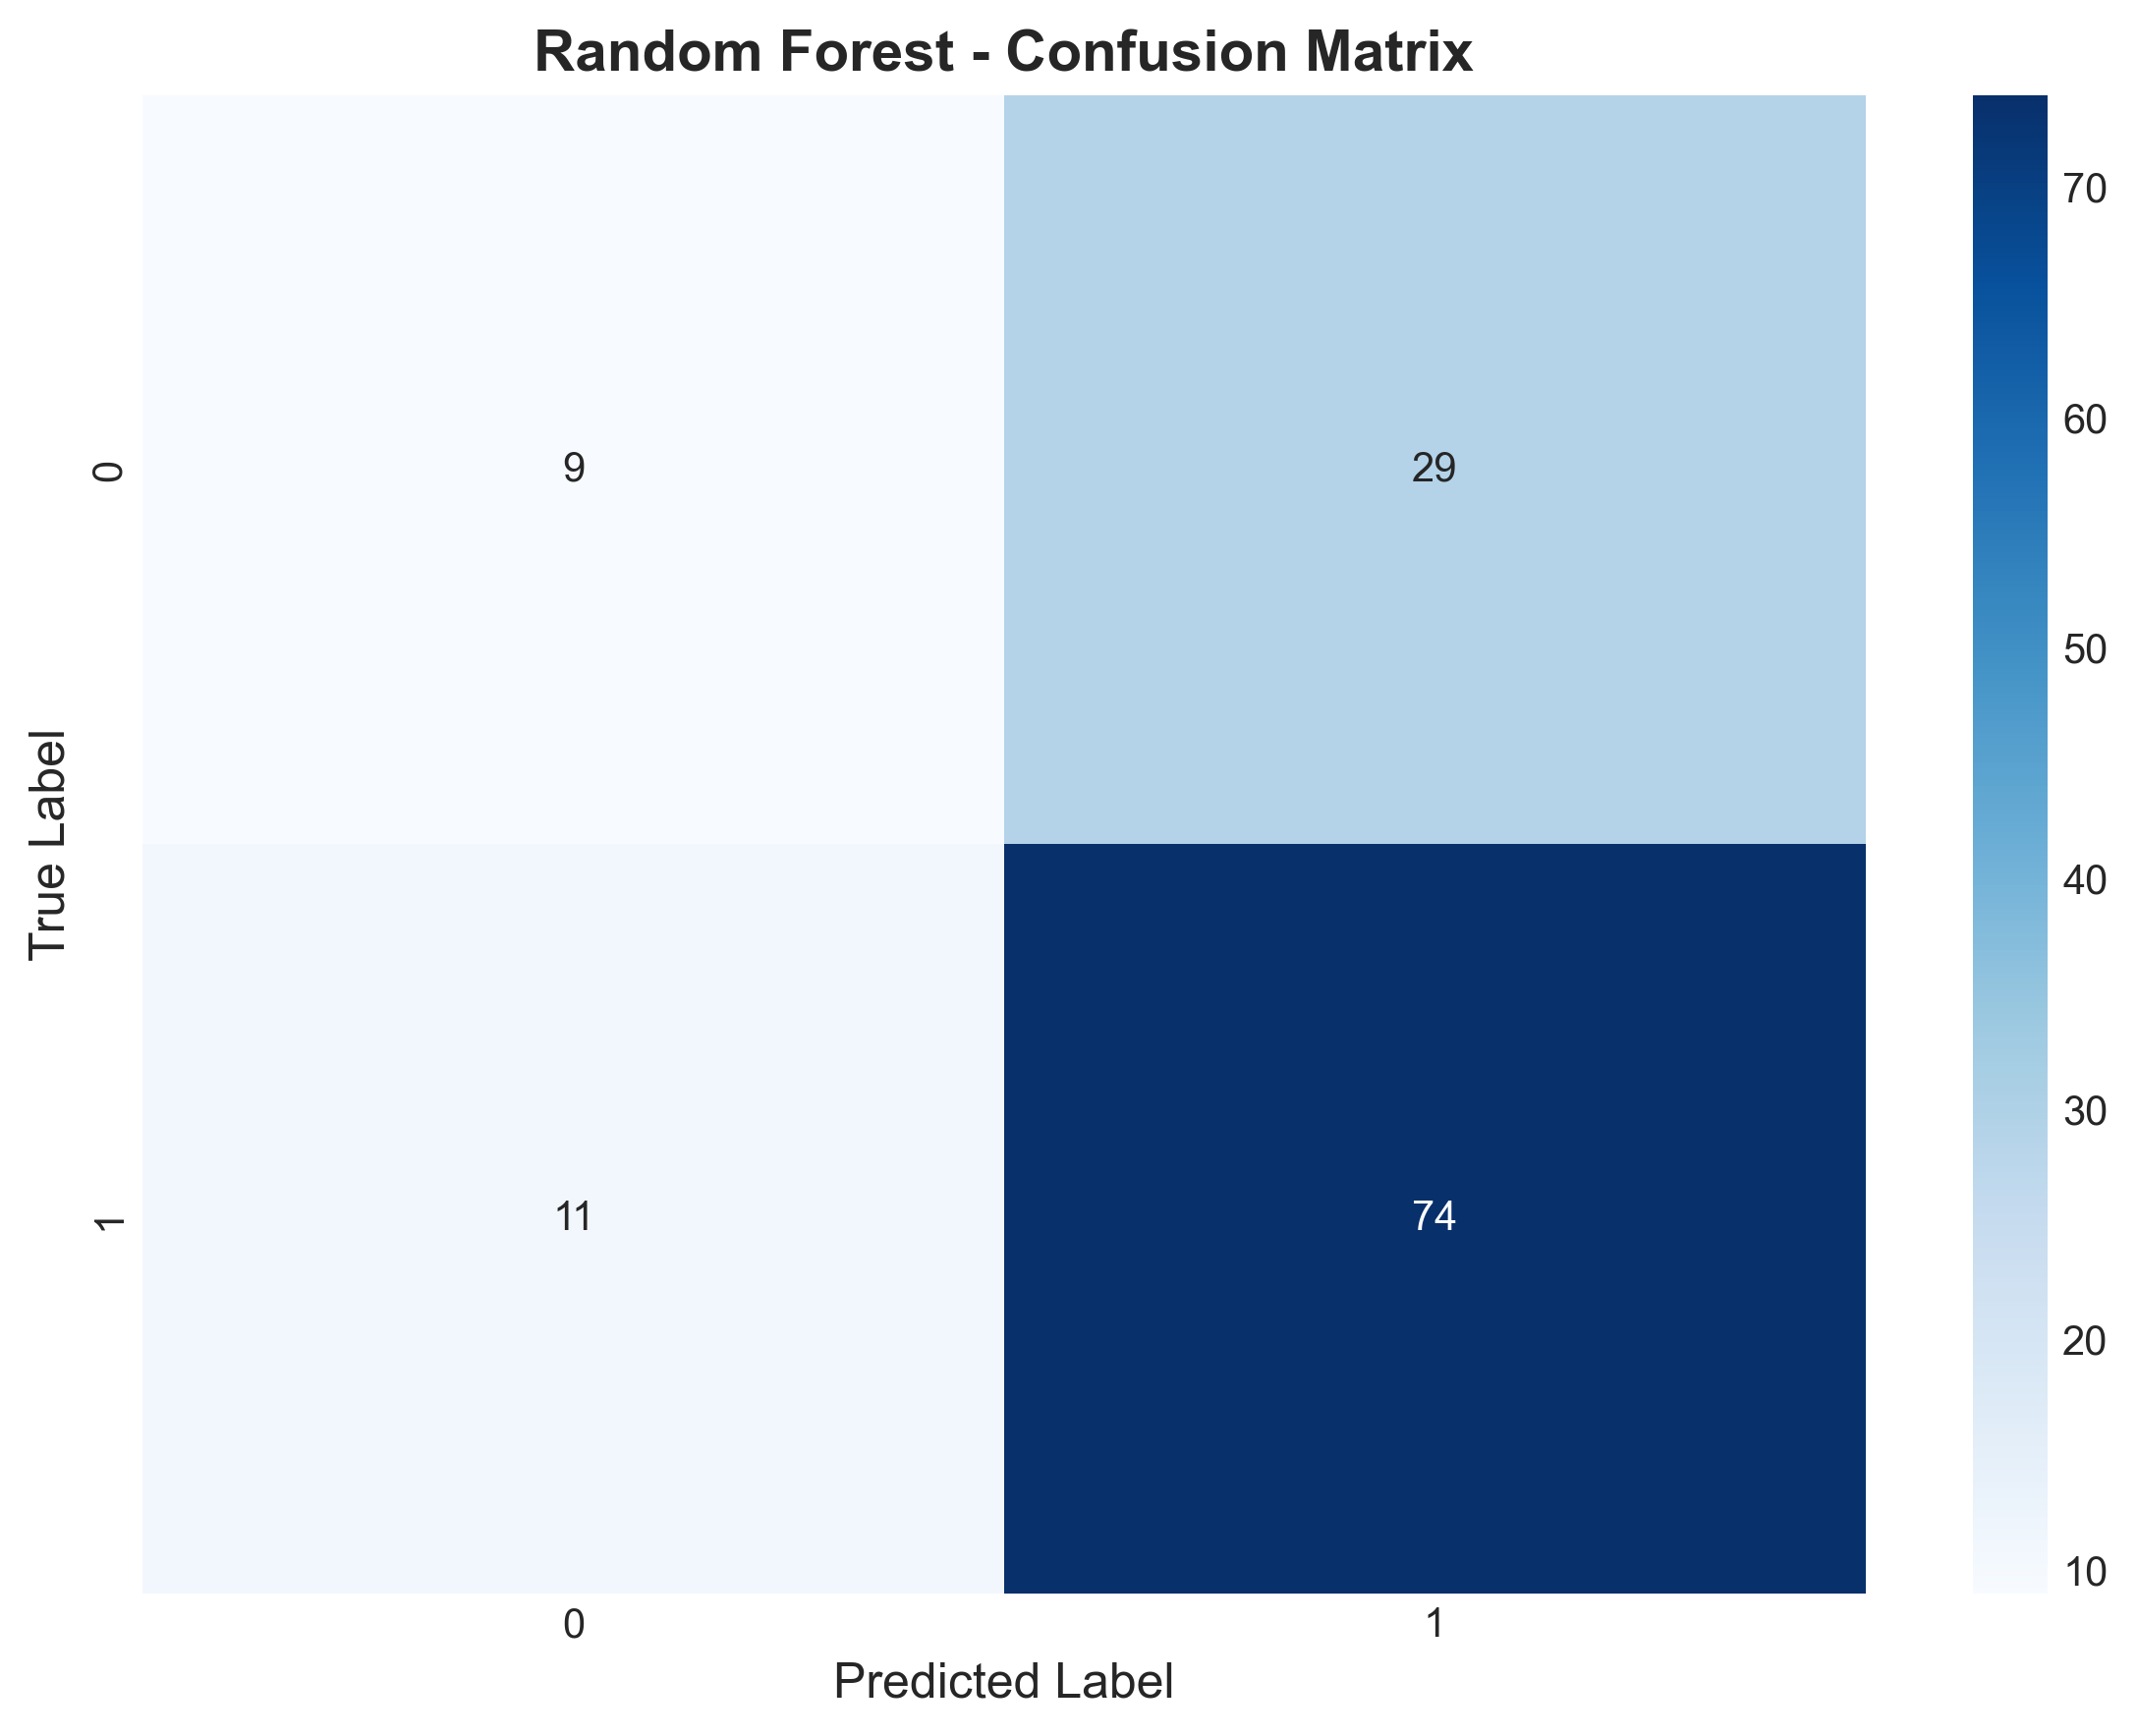
\includegraphics[width=\textwidth]{img/confusion_matrix_rf.png}
\small Random Forest
\end{center}

\column{0.5\textwidth}
\begin{center}
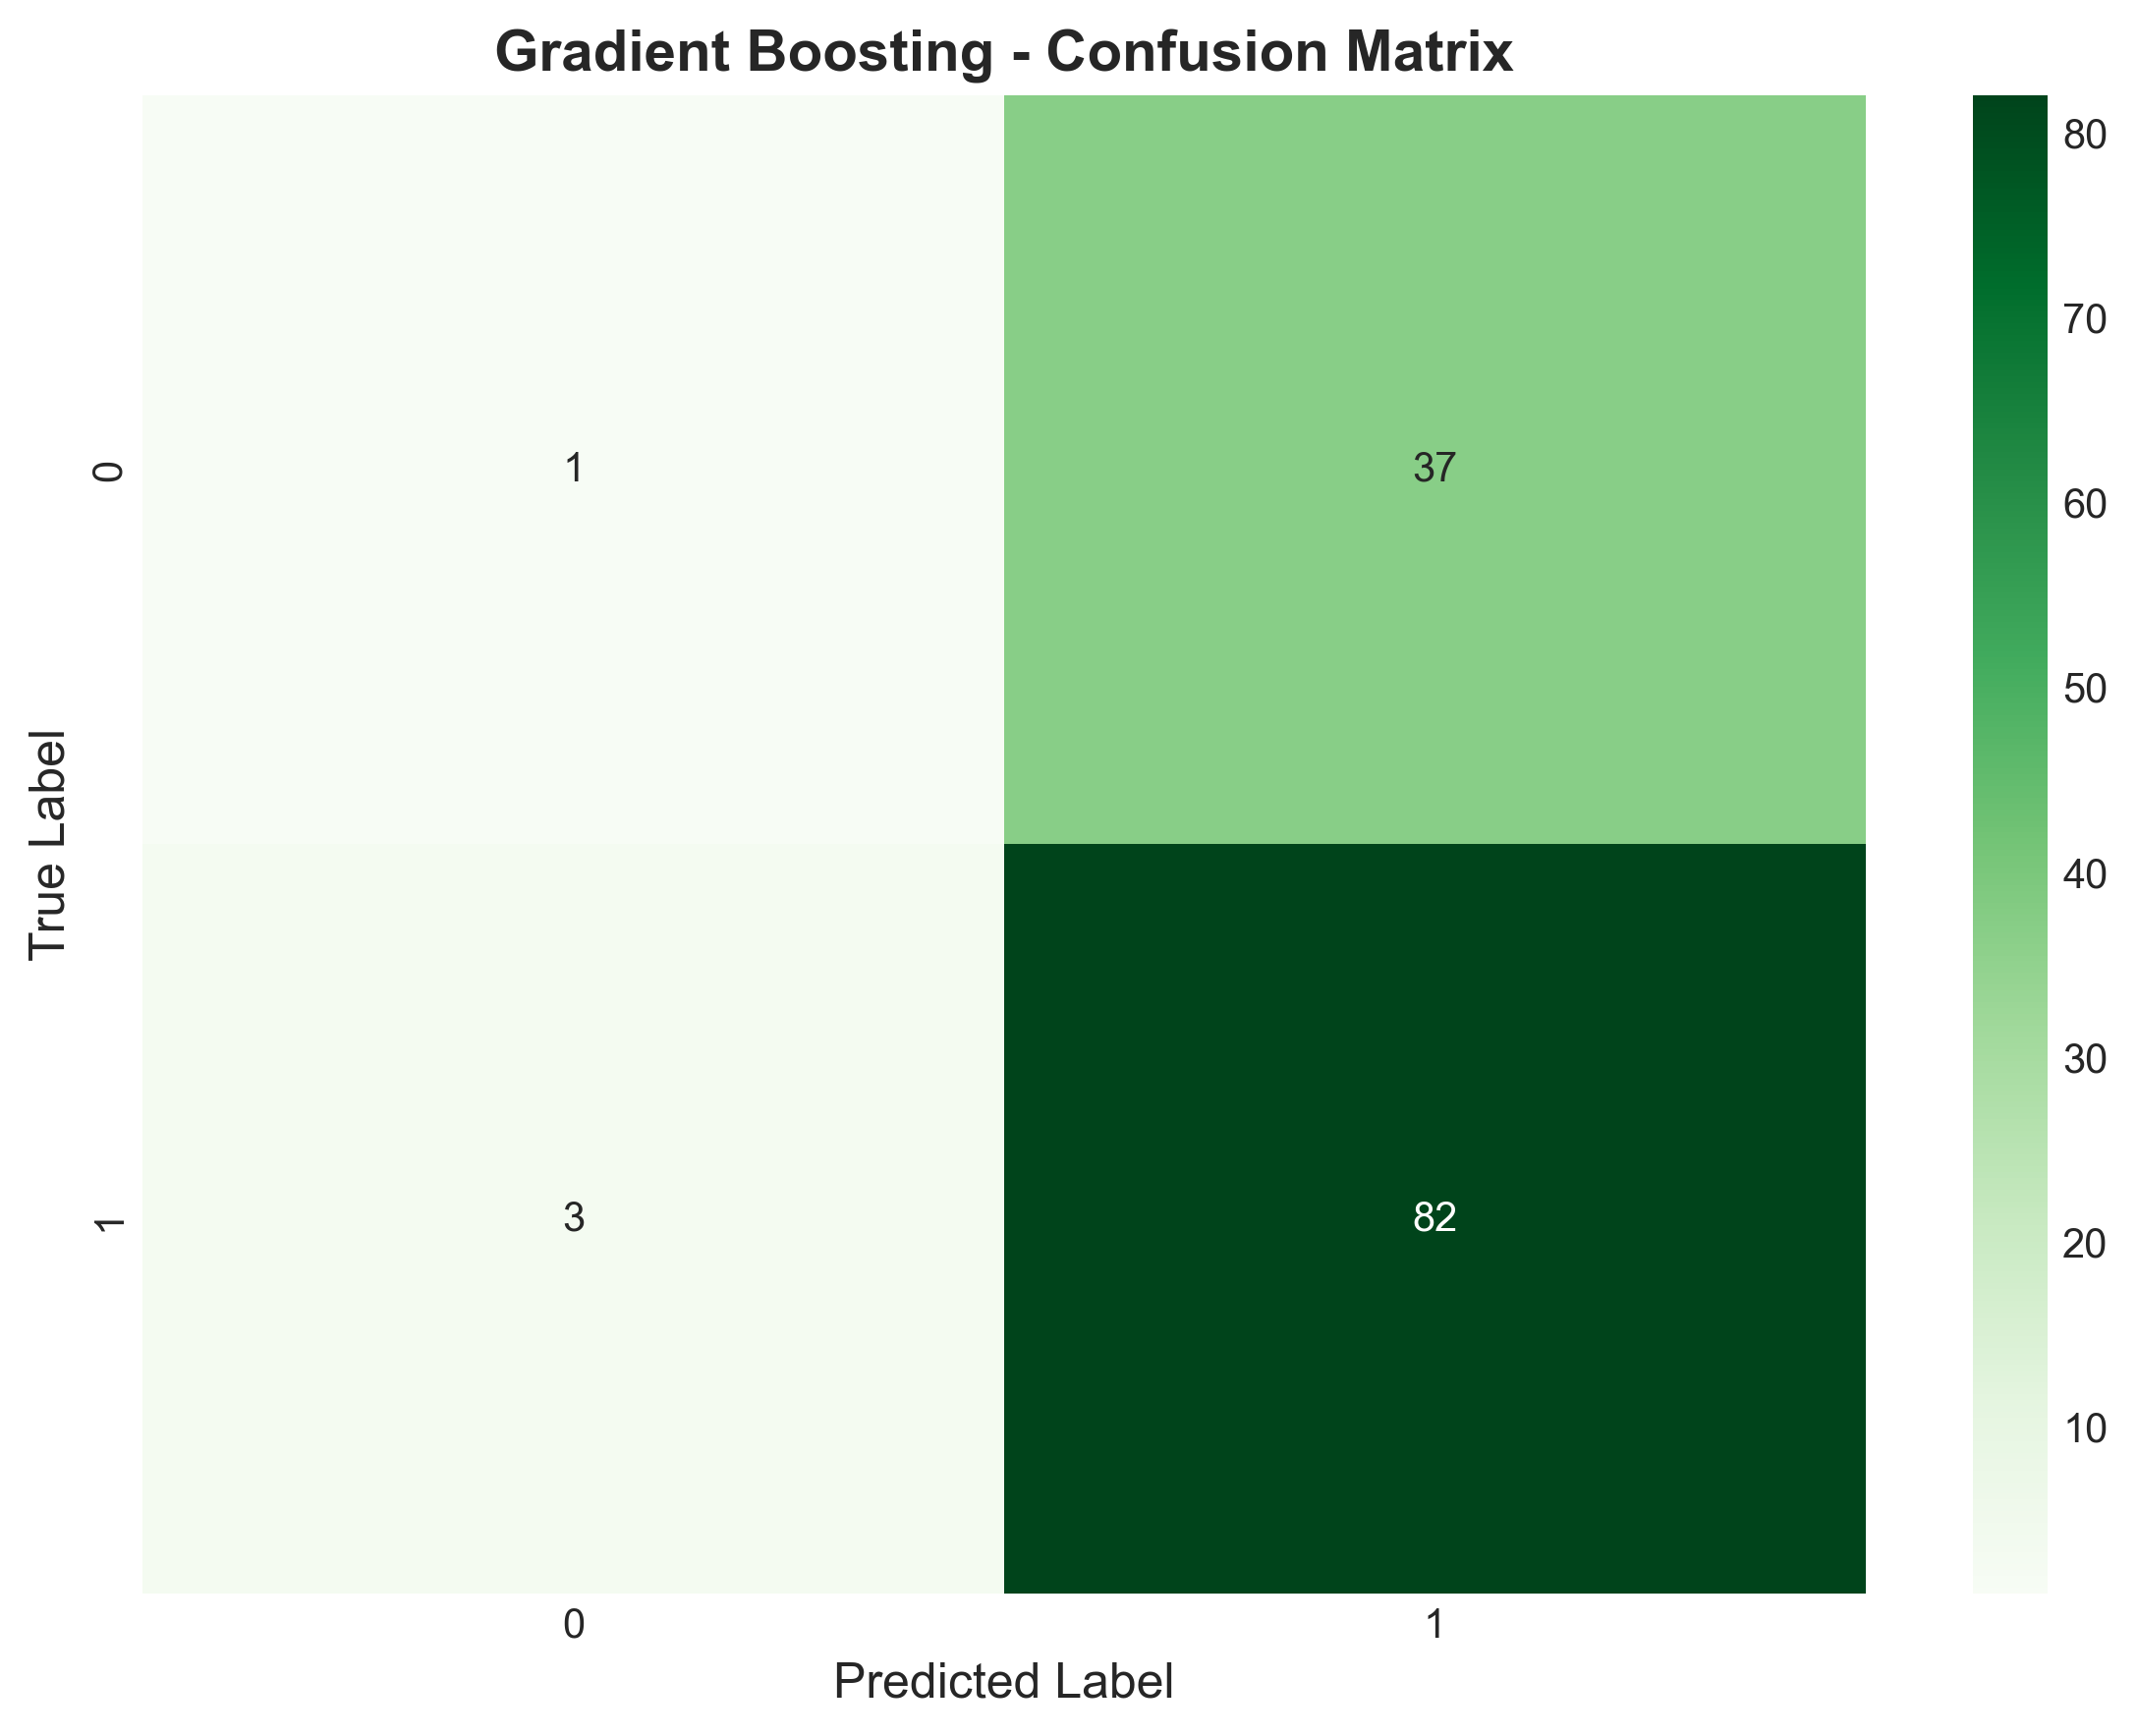
\includegraphics[width=\textwidth]{img/confusion_matrix_gb.png}
\small Gradient Boosting
\end{center}
\end{columns}
\begin{block}{تحلیل}
\begin{itemize}
\item RF: Precision بالاتر (کاهش False Positive)
\item GB: Recall بالاتر (شناسایی بیشتر True Positive)
\end{itemize}
\end{block}
\end{frame}

\begin{frame}{منحنی‌های ارزیابی}
\begin{columns}
\column{0.5\textwidth}
\begin{center}
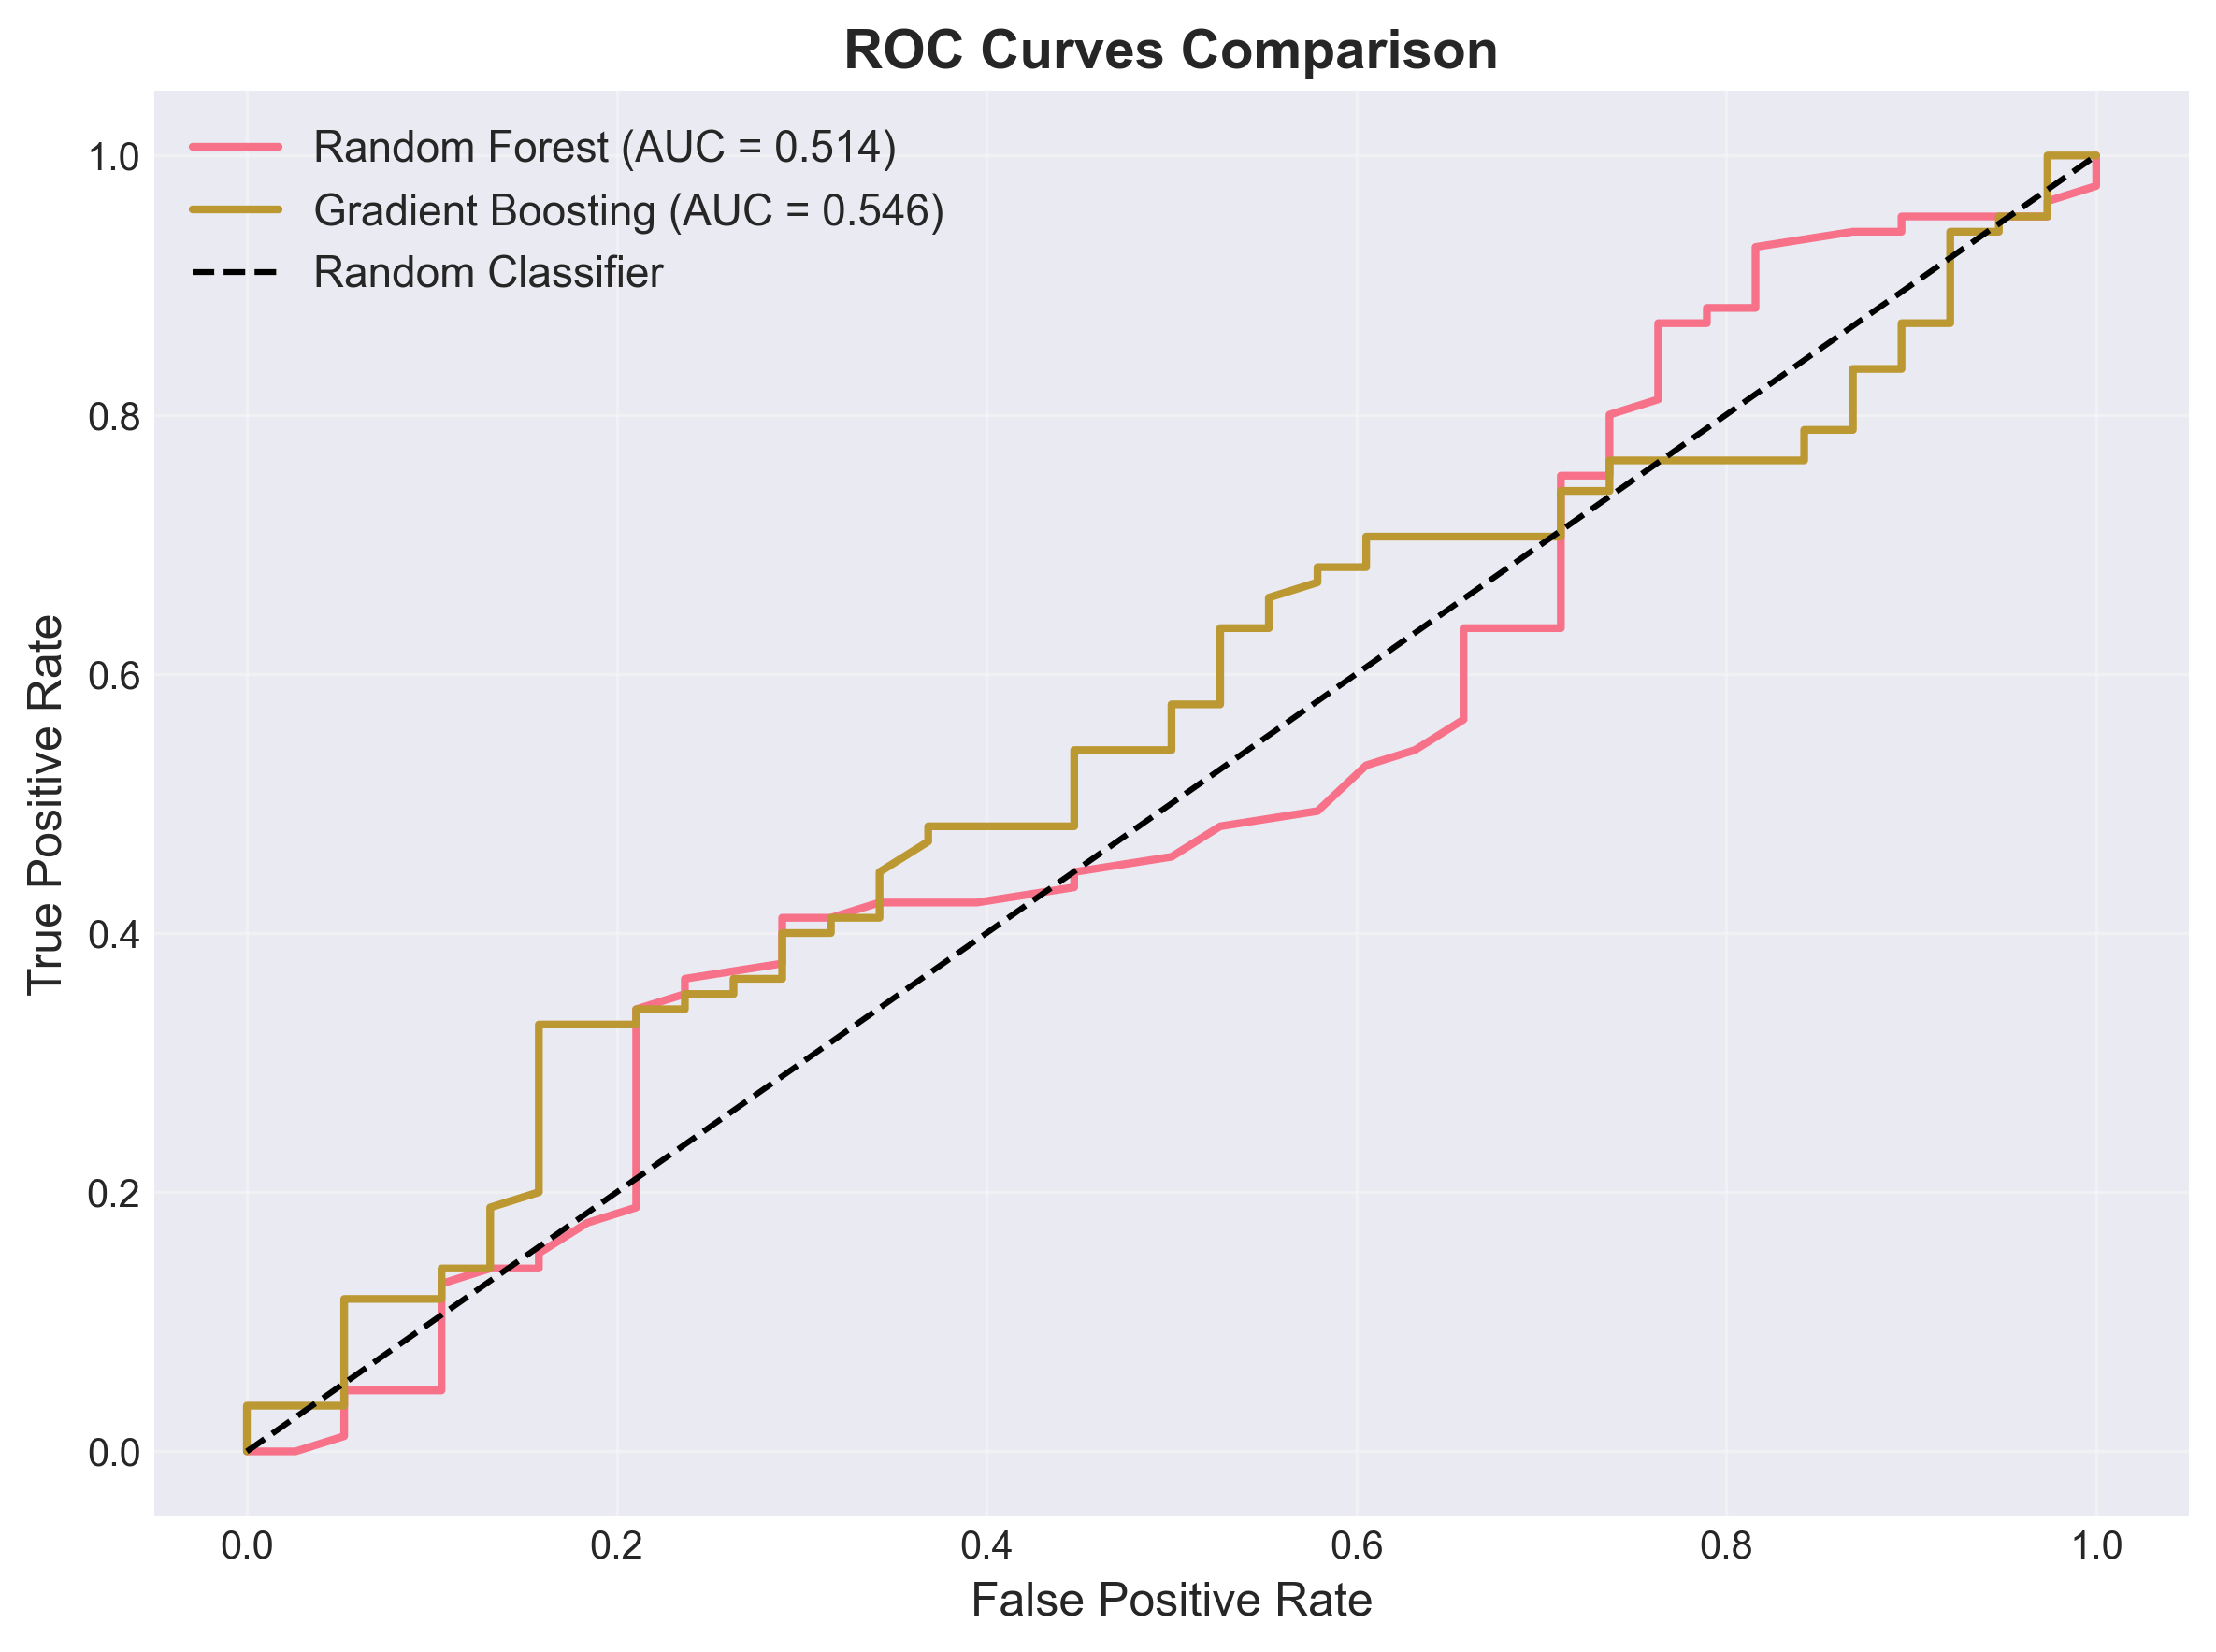
\includegraphics[width=\textwidth]{img/roc_curves.png}
\small منحنی ROC
\end{center}

\column{0.5\textwidth}
\begin{center}
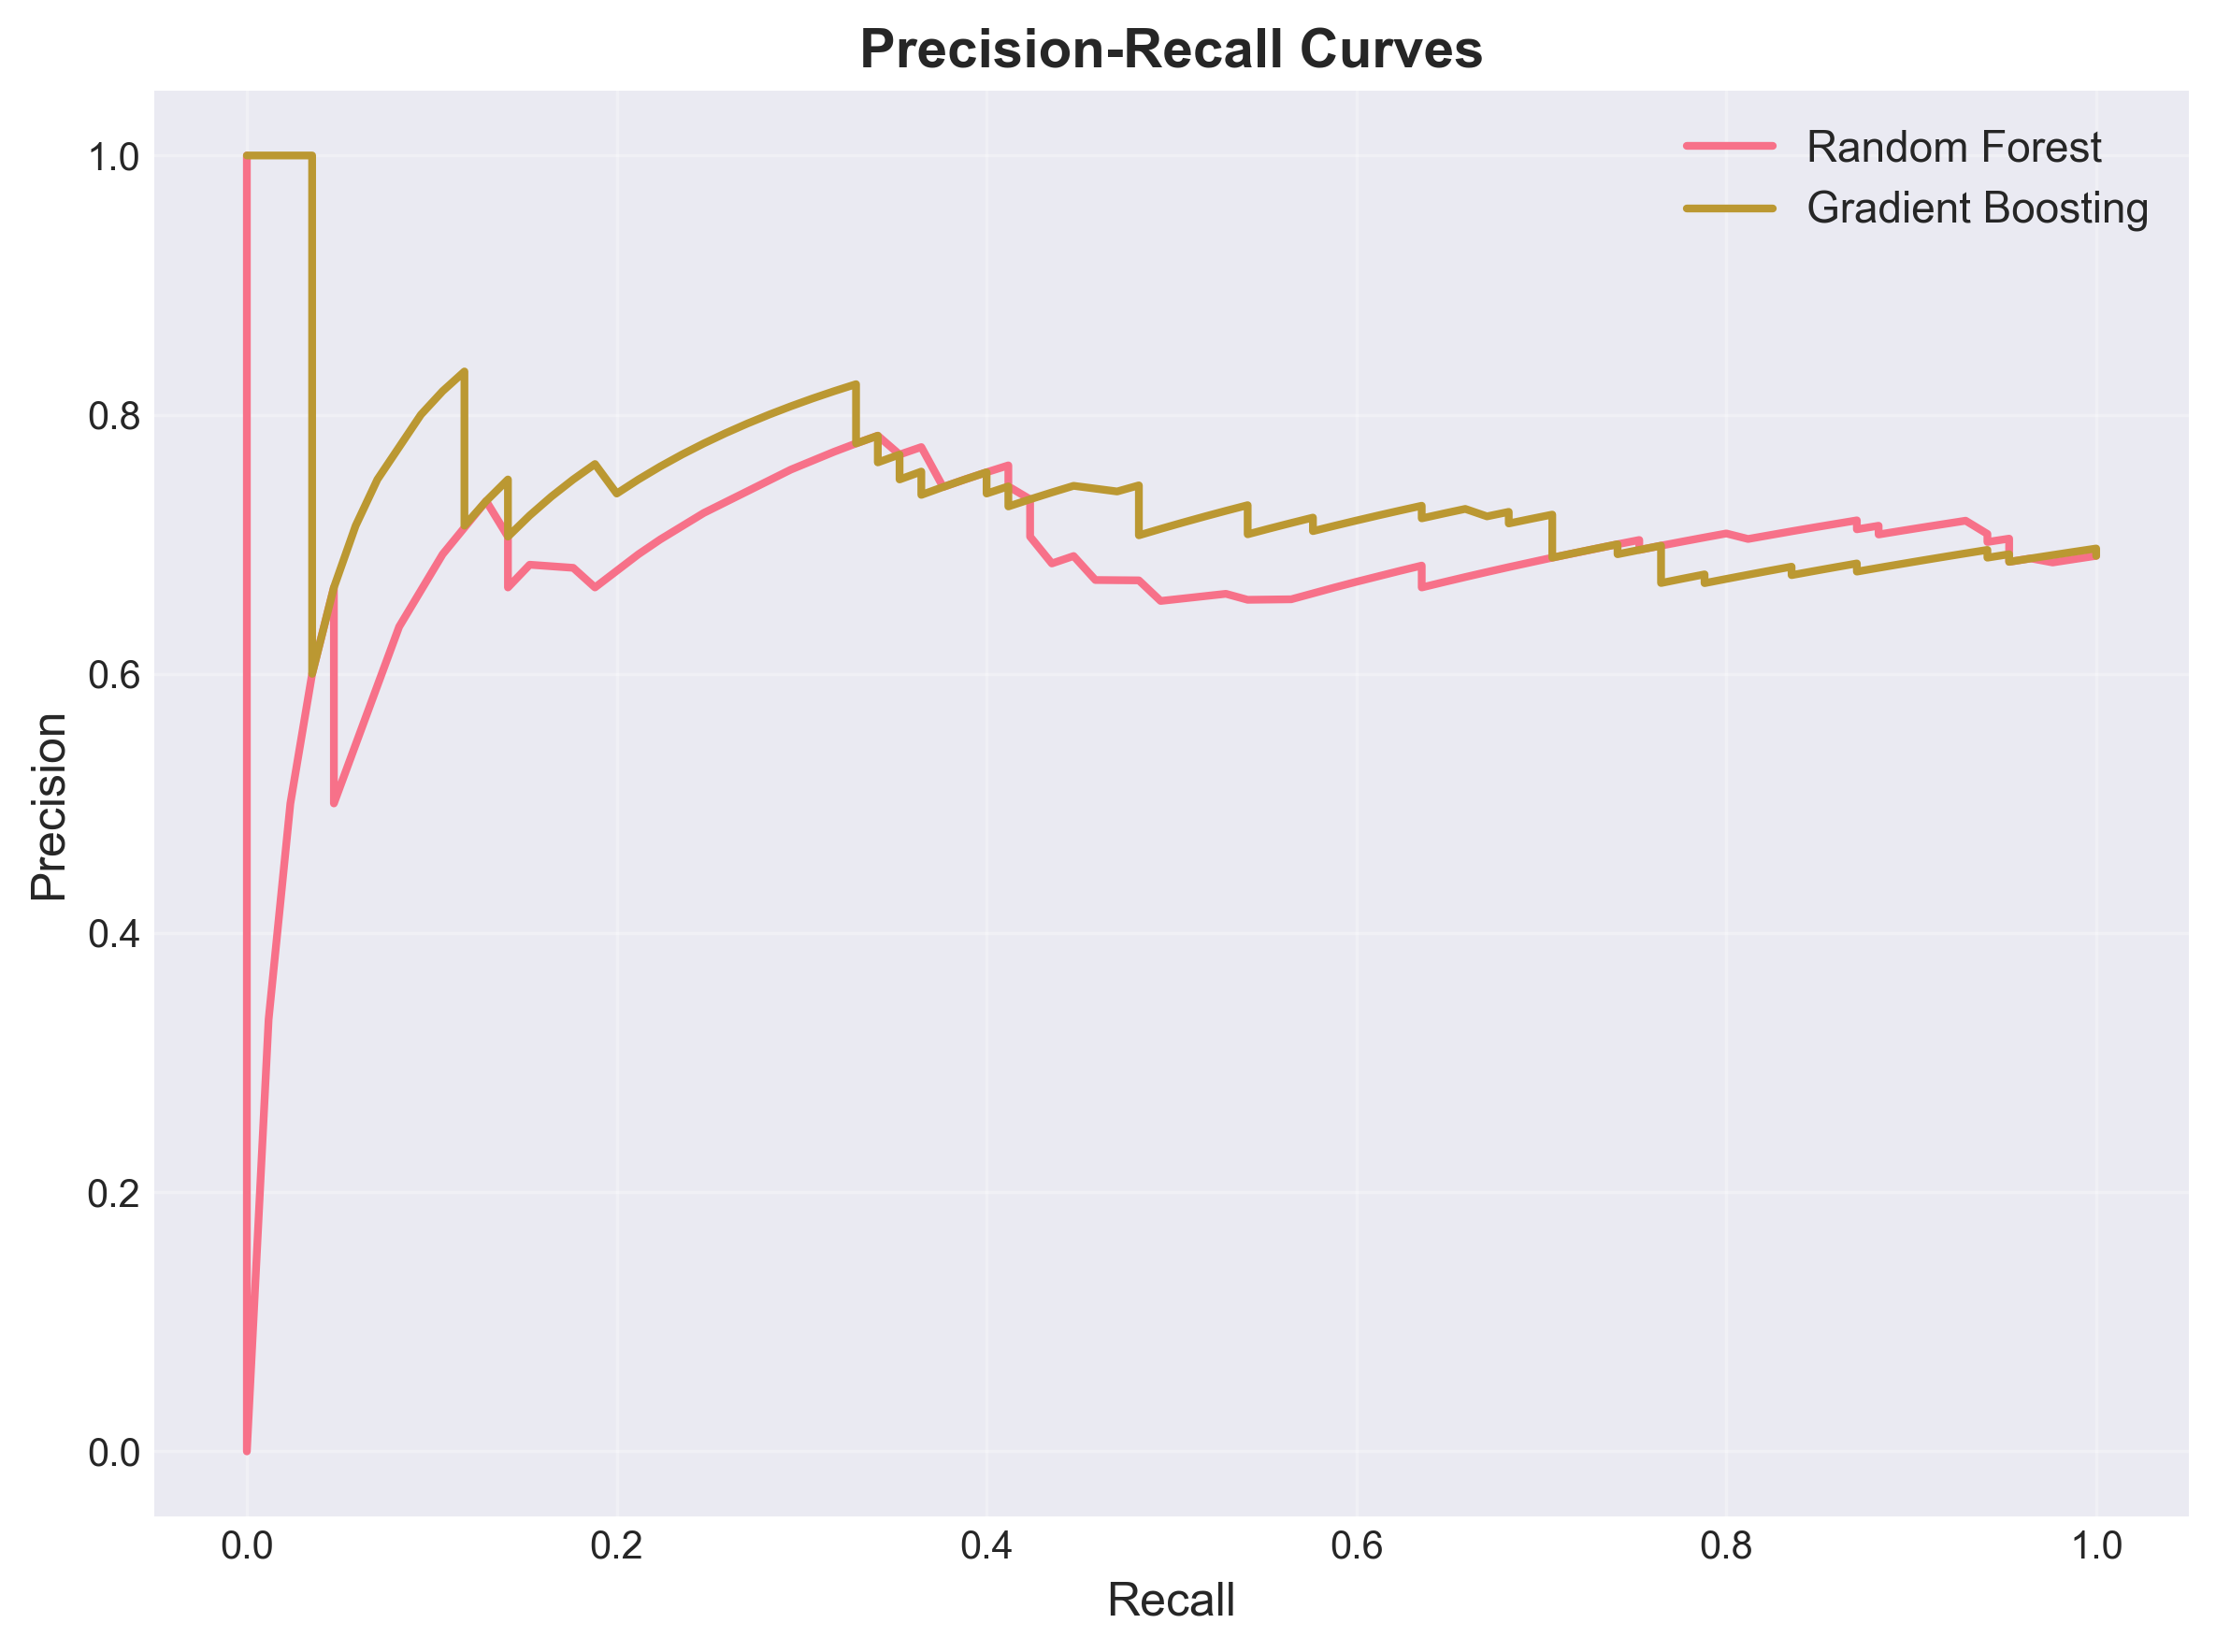
\includegraphics[width=\textwidth]{img/precision_recall_curves.png}
\small منحنی Precision-Recall
\end{center}
\end{columns}
\end{frame}

\begin{frame}{اهمیت ویژگی‌ها و مقایسه معیارها}
\begin{columns}
\column{0.5\textwidth}
\begin{center}
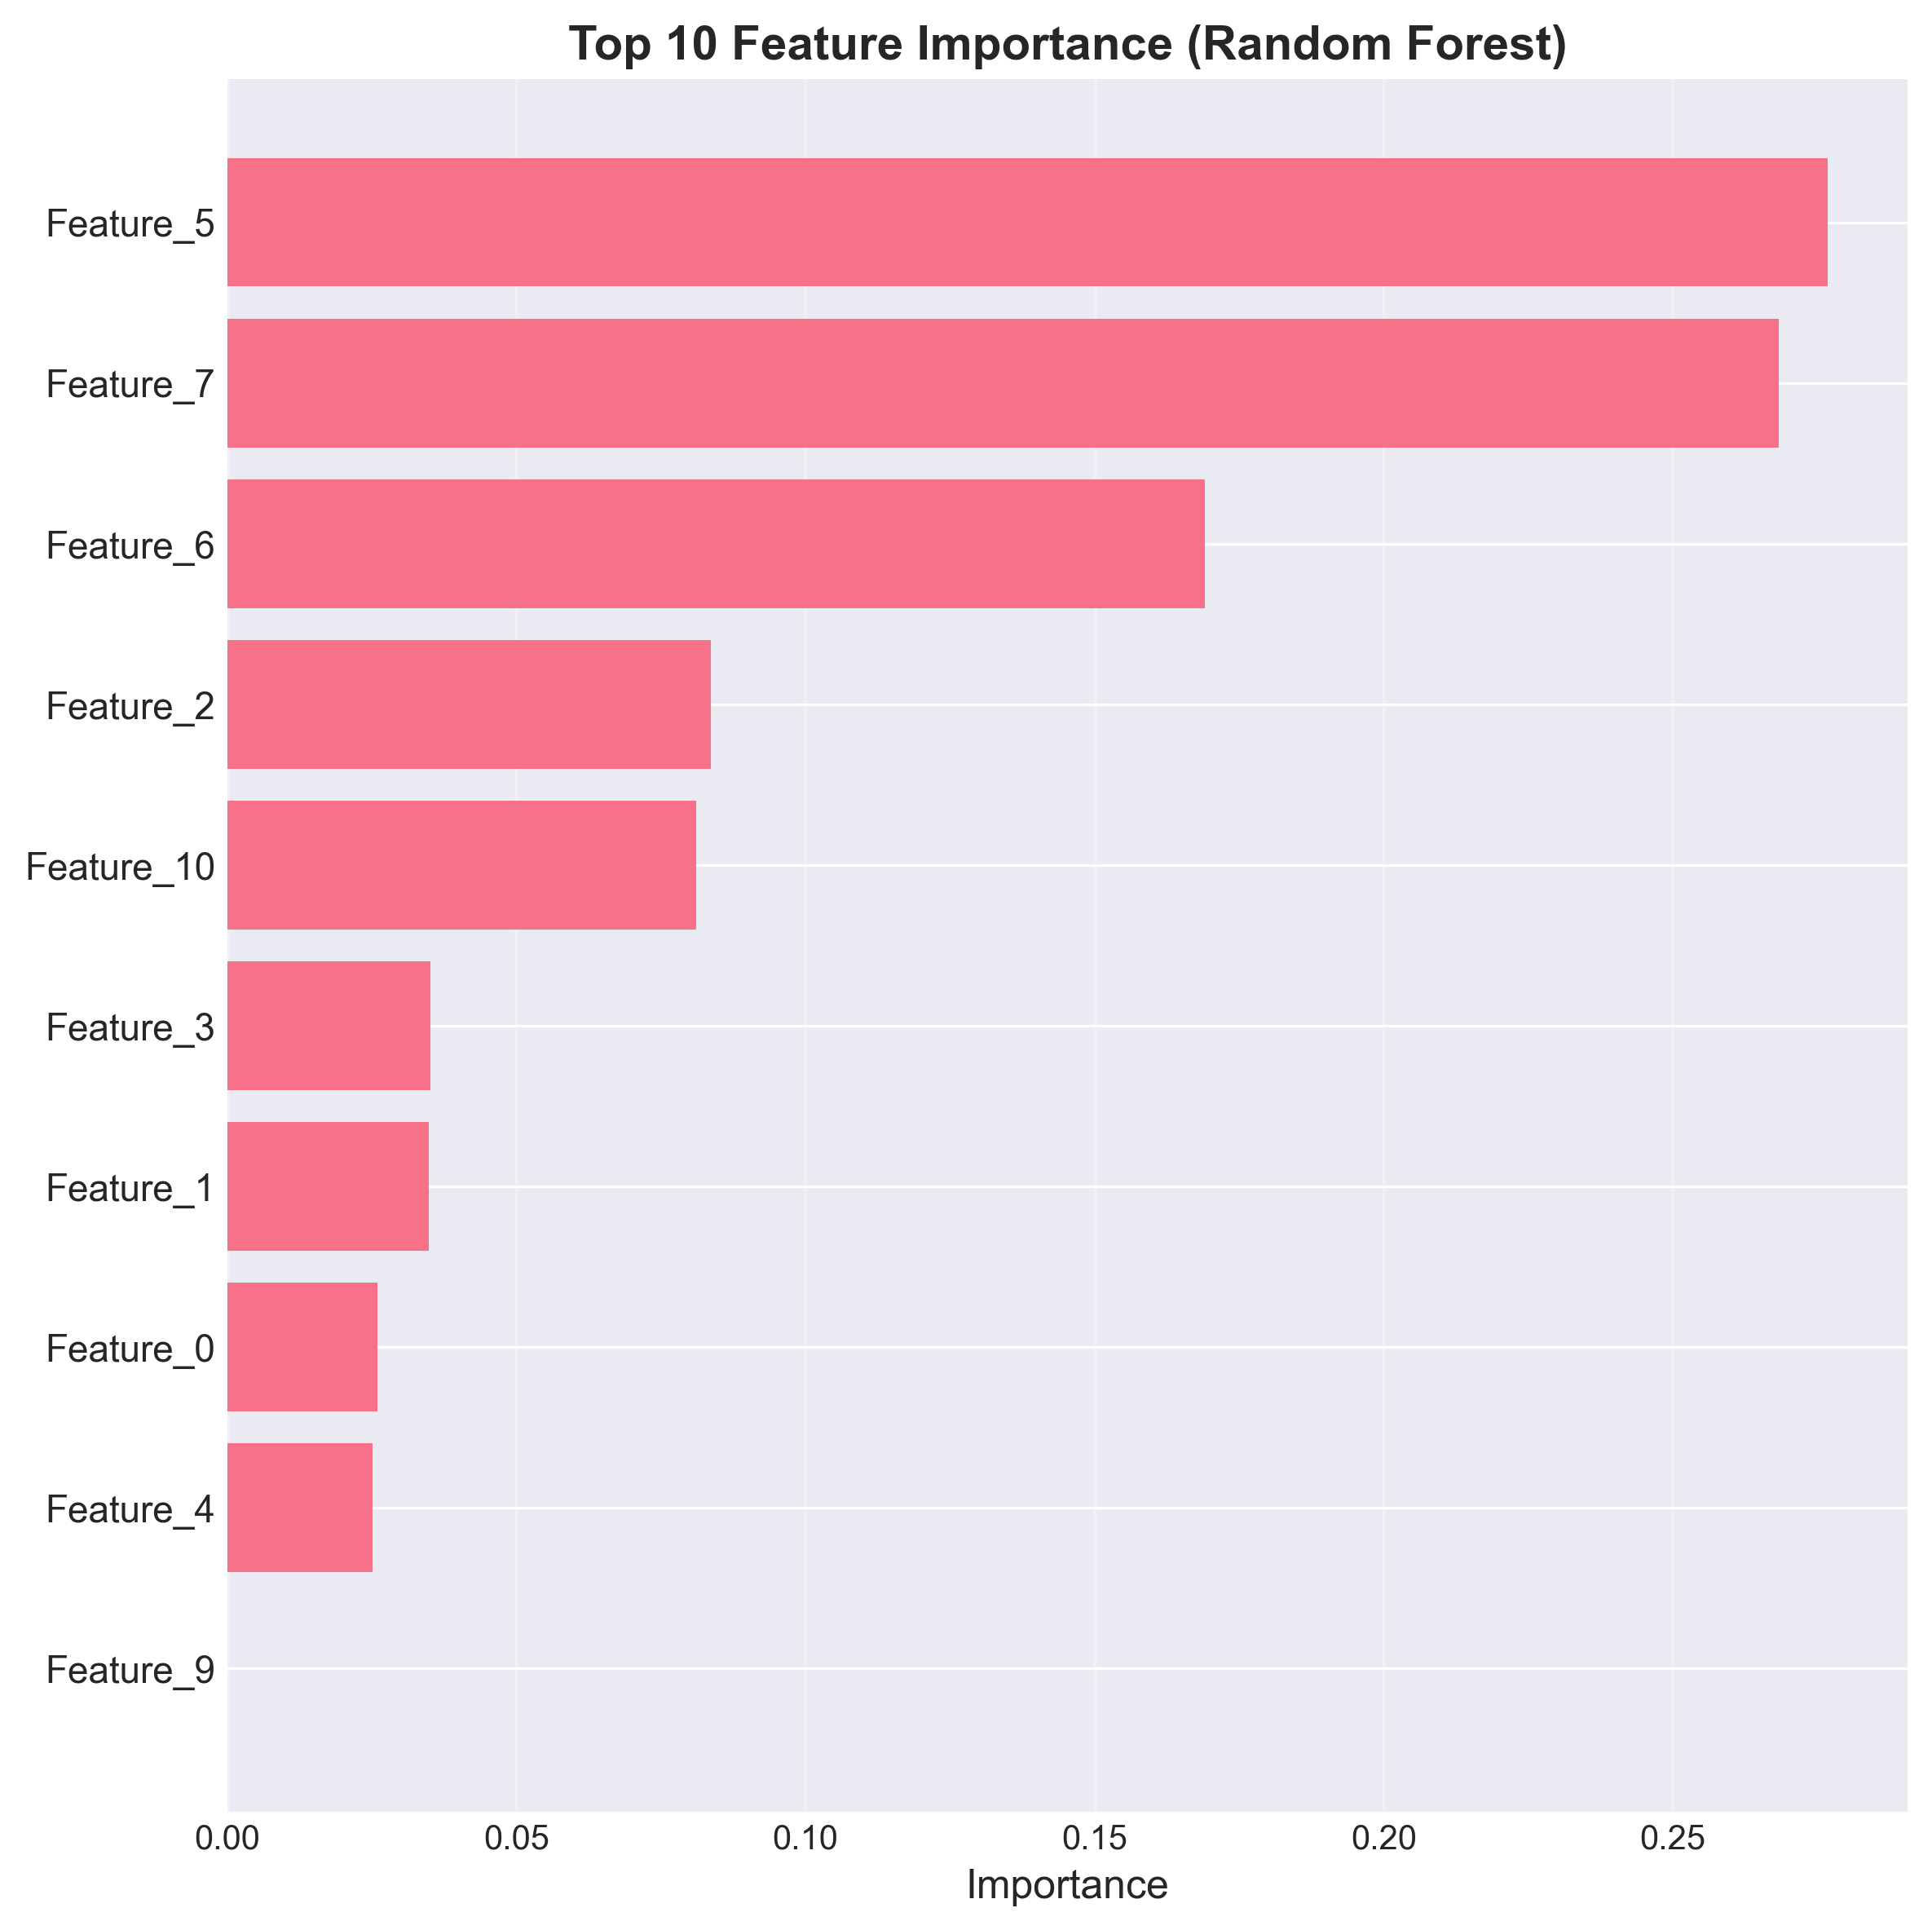
\includegraphics[width=\textwidth]{img/feature_importance.png}
\small اهمیت ویژگی‌ها
\end{center}

\column{0.5\textwidth}
\begin{center}
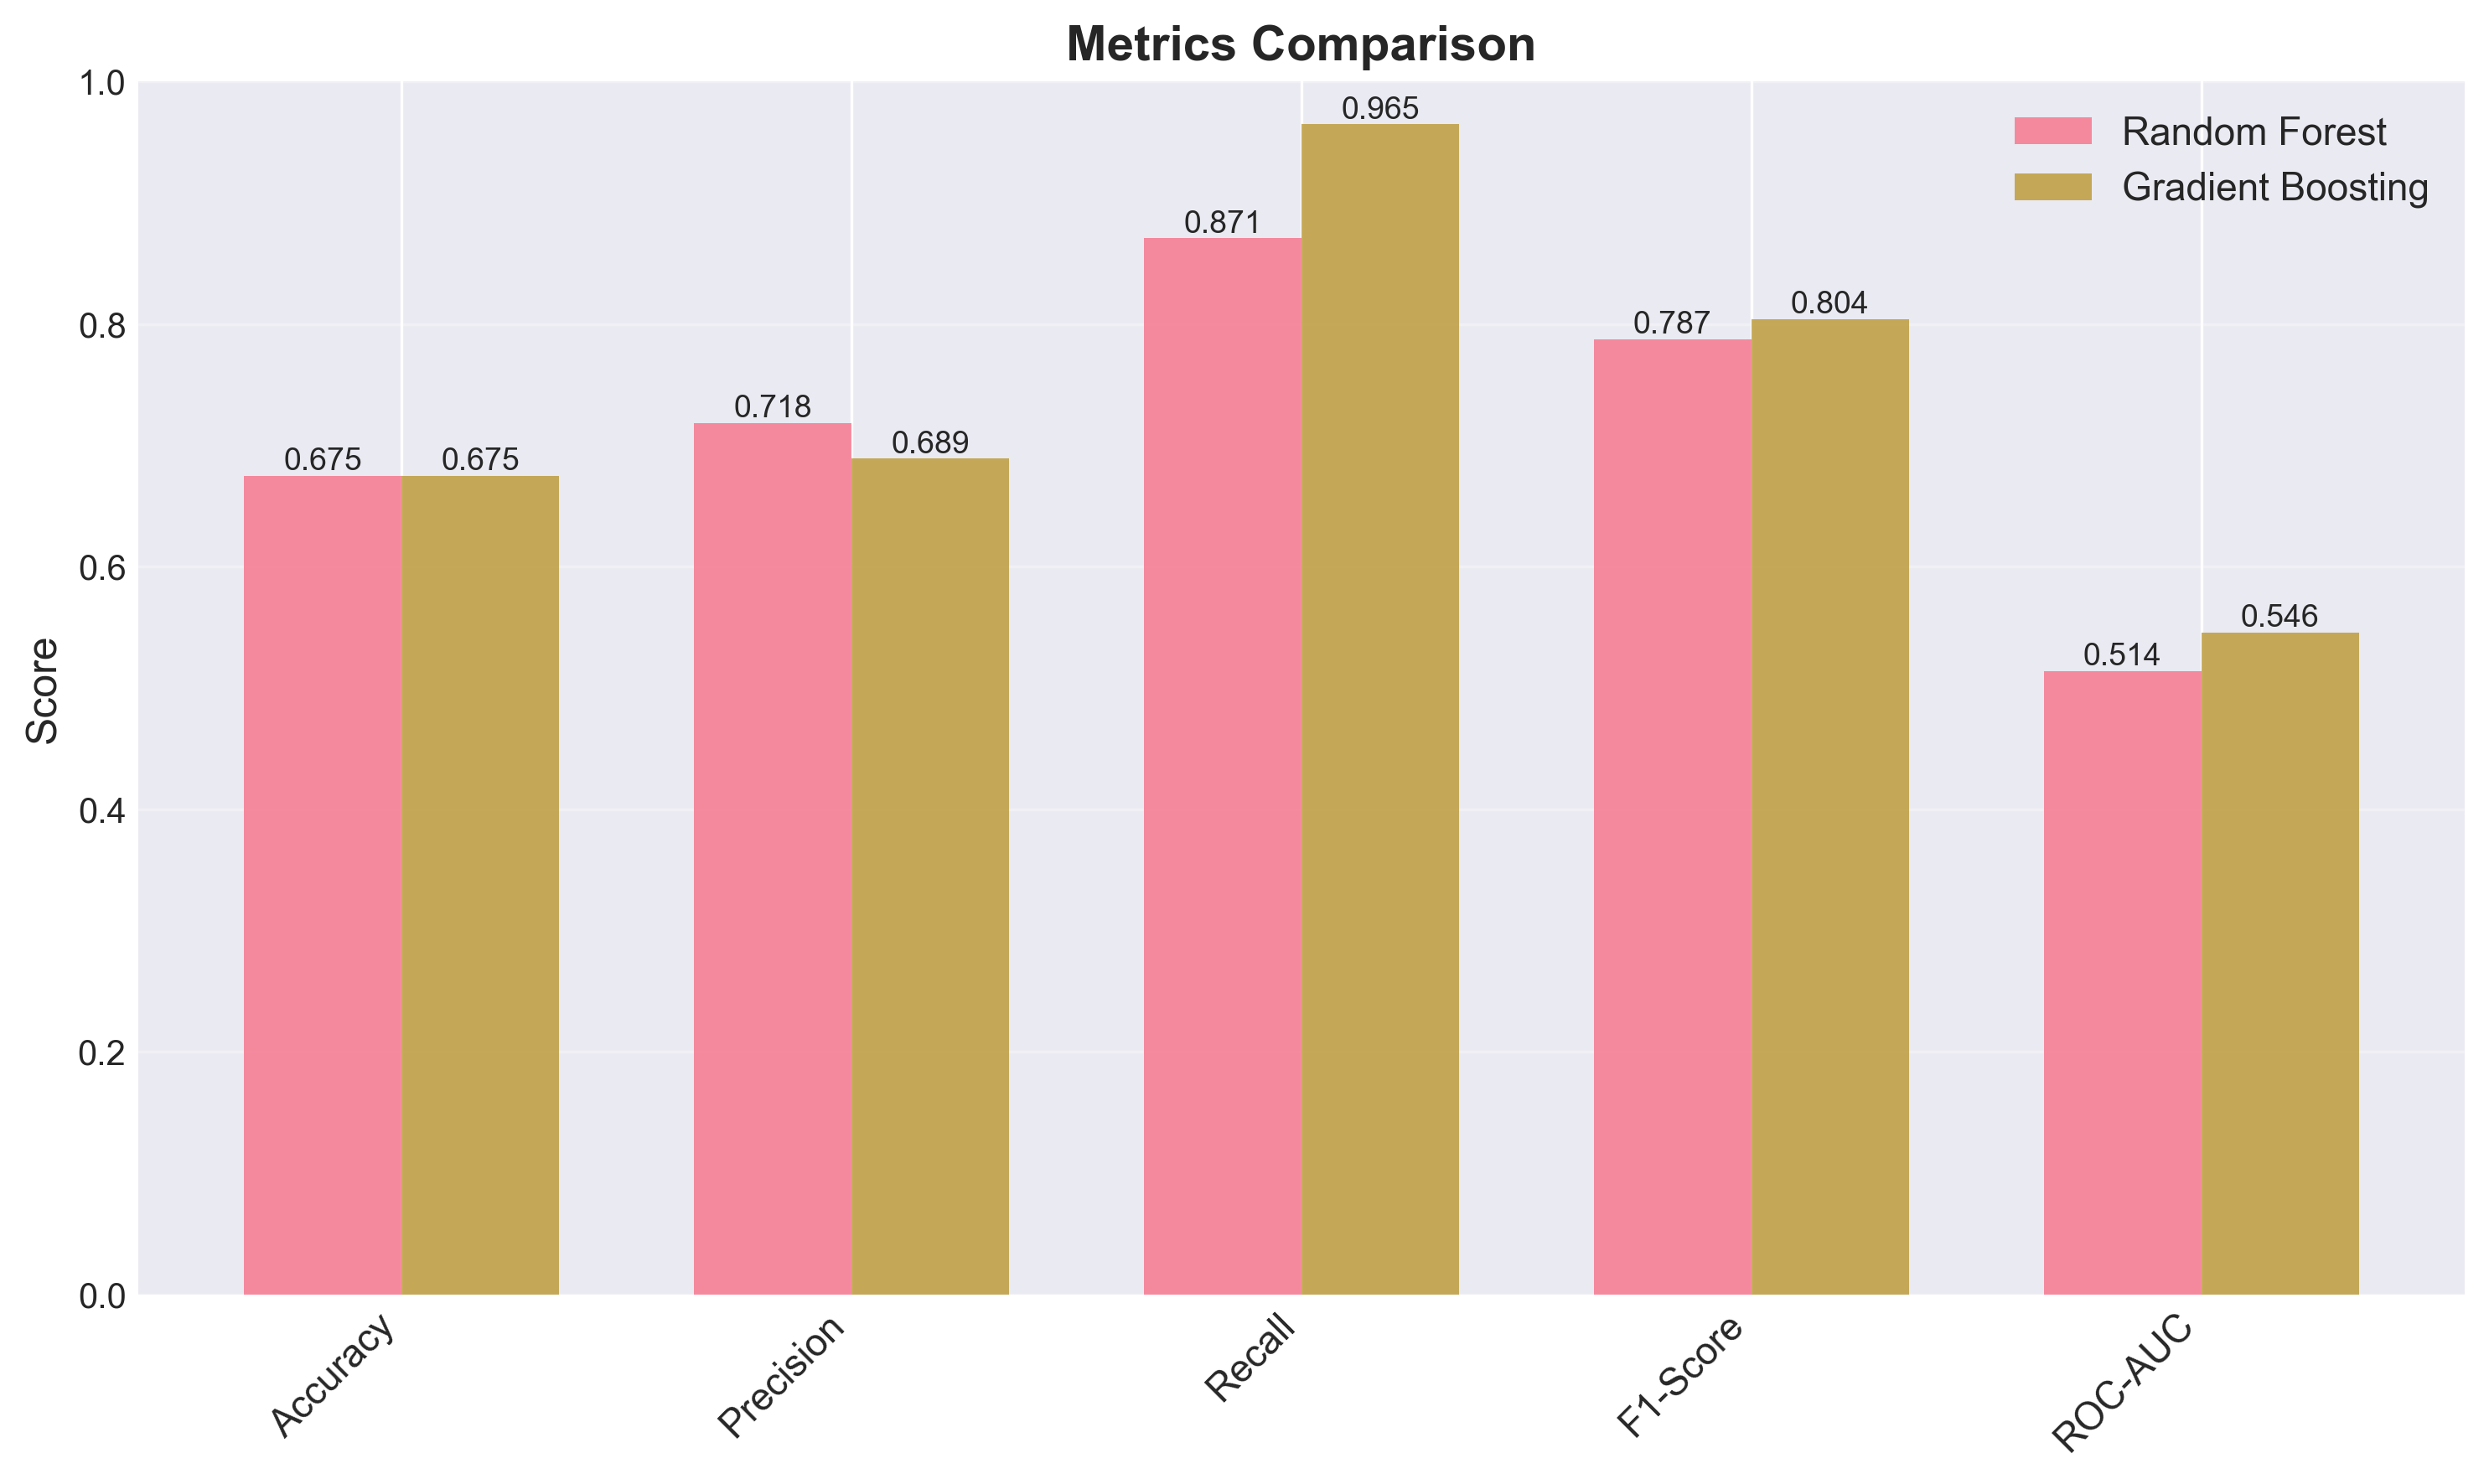
\includegraphics[width=\textwidth]{img/metrics_comparison.png}
\small مقایسه معیارها
\end{center}
\end{columns}
\end{frame}

\begin{frame}{بخش ۶: تحلیل ویژگی‌ها}
\begin{block}{اهمیت ویژگی‌ها (Random Forest)}
\begin{enumerate}
\item \textbf{Credit\_History} (مهم‌ترین)
\item Applicant\_Income
\item Loan\_Amount
\item Coapplicant\_Income
\item سایر ویژگی‌ها
\end{enumerate}
\end{block}

\begin{block}{نتیجه کلیدی}
\begin{itemize}
\item Credit\_History مهم‌ترین ویژگی است
\item با نتایج سوال ۱ مطابقت دارد
\item سایر ویژگی‌ها نقش کمتری دارند
\end{itemize}
\end{block}
\end{frame}


% ============================================
% CONCLUSION
% ============================================
\section{نتیجه‌گیری}

\begin{frame}{خلاصه نتایج}
\begin{block}{سوال ۱: انتخاب ویژگی}
\begin{itemize}
\item هر دو الگوریتم (PSO و GA) ویژگی \textcolor{important}{\textbf{Credit\_History}} را انتخاب کردند
\item دقت: \textcolor{highlight}{\textbf{۸۰.۶۷\%}} با تنها یک ویژگی
\item کاهش ابعاد: \textcolor{success}{\textbf{۹۰.۹\%}}
\end{itemize}
\end{block}

\begin{block}{سوال ۲: خوشه‌بندی}
\begin{itemize}
\item \textcolor{success}{\textbf{DBSCAN}} بهترین عملکرد را داشت
\item Silhouette Score: \textcolor{important}{\textbf{۰.۵۲۹۶}}
\item شناسایی ۴ خوشه و ۳۳\% نقاط نویز
\end{itemize}
\end{block}
\end{frame}

\begin{frame}{خلاصه نتایج (ادامه)}
\begin{block}{سوال ۳: یادگیری Q}
\begin{itemize}
\item بررسی نظری الگوریتم یادگیری Q
\item تحلیل معادله و پارامترها
\item شناسایی مسائل همگرایی و راه‌حل‌ها
\end{itemize}
\end{block}

\begin{block}{پروژه نهایی: خط لوله ML}
\begin{itemize}
\item پیاده‌سازی کامل از پیش‌پردازش تا ارزیابی
\item Gradient Boosting: F1-Score = \textcolor{highlight}{\textbf{۸۰.۳۹\%}}
\item Random Forest: Precision = \textcolor{important}{\textbf{۷۱.۸۴\%}}
\item \textcolor{success}{\textbf{Credit\_History}} تأیید شد به عنوان مهم‌ترین ویژگی
\end{itemize}
\end{block}
\end{frame}

\begin{frame}{دستاوردهای کلیدی}
\begin{block}{دستاوردهای اصلی}
\begin{itemize}
\item کاهش موفق ابعاد از ۱۱ به ۱ ویژگی با حفظ دقت بالا
\item شناسایی ساختار خوشه‌ای پیچیده با DBSCAN
\item تحلیل جامع نظری یادگیری تقویتی
\item پیاده‌سازی خط لوله کامل با عملکرد مناسب
\end{itemize}
\end{block}

\begin{block}{کاربردهای عملی}
\begin{itemize}
\item سیستم پیش‌بینی وام با دقت بالا
\item تقسیم‌بندی مشتریان برای بازاریابی هدفمند
\item درک عمیق از الگوریتم‌های یادگیری تقویتی
\end{itemize}
\end{block}
\end{frame}

\begin{frame}{پیشنهادات بهبود}
\begin{block}{برای انتخاب ویژگی}
\begin{itemize}
\item تست با مقادیر مختلف $\alpha$
\item استفاده از روش‌های دیگر مانند RFE
\end{itemize}
\end{block}

\begin{block}{برای خوشه‌بندی}
\begin{itemize}
\item تست با داده‌های بیشتر
\item استفاده از الگوریتم‌های ترکیبی
\end{itemize}
\end{block}

\begin{block}{برای خط لوله ML}
\begin{itemize}
\item استفاده از SMOTE برای مدیریت عدم تعادل
\item مهندسی ویژگی‌های جدید
\item تست مدل‌های دیگر مانند XGBoost
\item تنظیم آستانه تصمیم‌گیری
\end{itemize}
\end{block}
\end{frame}

% Thank you slide
\begin{frame}
\begin{center}
\Huge \textbf{سپاسگزاریم}

\vspace{1cm}

\Large سوالات؟
\end{center}
\end{frame}

\end{document}

